\makeatletter 
\renewcommand{\thefigure}{A\@arabic\c@figure} 
\makeatletter 
\renewcommand{\thetable}{A\@arabic\c@table} 
\makeatletter 
\renewcommand{\thesection}{A\@arabic\c@section} 
\newpage
\section{SEPP}
SEPP (SAT\'e-enabled phylogenetic
placement)  is used for one of 
the  major algorithmic
steps which TIPP.
We describe SEPP's strategy briefly here, but
see \cite{Mirarab2012} for full details.
We let $A$ be
the  reference alignment and $T$ the reference tree on the set $S$ of 
full-length sequences.

\noindent{\bf Step 1: Decomposition.}  
The parameters that govern the decomposition strategy are
$m_p$, the maximum size of the ``placement subsets", and
$m_a$, the maximum size of the ``alignment subsets".
SEPP requires that each alignment subset be a subset of
a placement subset, and so requires that $m_a \leq m_p$.
SEPP uses $T$ to
decompose the sequences in $S$ into 
disjoint placement subsets, and then decomposes
the placement subsets further (if $m_a < m_p$) into
disjoint alignment subsets, as follows.
SEPP finds a centroid edge in $T$ (one that
separates the leaf set into two sets of
approximately equal size), and breaks the tree accordingly into two subtrees.
For each resulting subtree that contains more than $m_p$ leaves, 
SEPP recursively repeats this decomposition.
This produces a partition of $S$  into subsets $S_1, S_2, \ldots, S_k$,
with each subset having at most $m_p$ elements.
If $m_a < m_p$, then the decomposition
process continues on any subset $S_i$ with more than $m_a$ leaves,
until each placement subset has been further partitioned into
disjoint
alignment subsets, each having at most $m_a$ leaves. 


\noindent{\bf Step 2: Compute Extended Alignment. }  
For a given alignment subset of sequences $S' \subset S$, 
we define $A'$ to be restriction of alignment $A$ to $S'$.
SEPP uses HMMER to compute an HMM $H'$ on $A'$ for each alignment subset
and to score $q$ with respect to each $H'$.
Thus, SEPP represents the backbone alignment with a set of
HMMs (a technique we call an ``HMM
Family).
HMMER produces measures of the fit between
each HMM and each query sequence called ``bit-scores" (discussed in
Section \ref{tipp:bitscores}).
Then,  for each query sequence $q$, the alignment
subset with the best bit-score is noted.
SEPP uses HMMER to align $q$ to the alignment
on the subset with the best bit-score, and
then extends the reference alignment $A$ on the full dataset to include $q$.
This is an ``extended alignment" for the query $q$;
thus, each query sequence $q$ gives rise to a different extended
alignment with $|S|+1$ sequences.

\noindent{\bf Step 3: Placement. }
The query sequence $q$ is placed in the reference tree
$T$
using the  preferred  placement method.
The current implementation of SEPP enables the use of both
pplacer and EPA for the placement of
fragments. EPA and pplacer 
have identical optimization criteria and
use very similar techniques:
both
place fragments to optimize maximum likelihood
using  
the GTRGAMMA model for DNA sequences or a selected protein model 
for AA sequences, and 
return a set of placements, each with
its confidence level. See Section \ref{supp:hmmer_epa} for more discussion
about EPA and pplacer, and a comparison of their
performance. 

As described, SEPP places fragments into the reference tree;
however, SEPP (and any
phylogenetic placement method) can be used to 
place fragments into any tree on the same set of sequences,
optimizing likelihood; this allows SEPP to use the
reference tree to divide the sequence dataset into
alignment subsets, and yet place 
the fragments into some other tree. 
This flexibility will be useful in developing TIPP.

\cite{Mirarab2012} found
settings for the
SEPP parameters that gave good accuracy in
reasonable time under a wide range of conditions; these were
$m_a=10$ and
$m_p=n$, where $n$ is the number of leaves in the reference alignment and tree.
Thus, small alignment subsets improve accuracy, and
placing in the entire tree improves accuracy.
However, when $n$ is very large, 
these settings are computationally expensive.
To reduce the computational challenges, SEPP limits the 
portion of the reference tree into which each query sequence can be placed;
this is the purpose of the parameter $m_p$.
Precisely, if the best alignment subset
for the query sequence is determined to be
$S^a$, 
then SEPP places $q$ into the subtree of
the reference tree defined by 
the leaves of $S^p$, where $S^p$ is the unique placement subset
containing $S^a$.
This defines a unique edge in the reference
tree into which to place the query sequence.
% (i.e. the subtree defined by the placement subset
%that includes the best-scoring alignment subset).

\section{TIPP on larger markers}\label{supp:large_marker}
We modified how we run TIPP on the bacterial 16S RNA
dataset due to the large number of taxa (9197),
as follows: we used the SAT\'{e} alignment
as the reference alignment, the
refined taxonomy as the reference tree, and rather
than placing into the entire refined taxonomy, we use
SEPP to decompose the refined taxonomy into both alignment
subsets and placement subsets using decomposition
parameters of $m_p=1000$ and $m_a=100$.  Thus, reads are
placed into subtrees of the 16S marker, each of which
contains at most 1000 leaves.


\section{Precision and Recall Comparisons and Statistical Significance}
In this section we compare techniques two at a time according to precision and recall.
For each comparison we show tables with differences between precision and recall values of the two techniques being compared,
and indicate whether the differences are statistically significant. 

\subsection{HMMER+pplacer versus HMMER+EPA}\label{supp:hmmer_epa}
Table \ref{tipp:difference.leaveout.rspb.pplacer.epa} shows that 
pplacer and EPA are indistinguishable in terms of both precision and recall
(i.e., the differences are not statistically significant).

\begin{table}[hptb]
\caption[Precision-Recall Differences between HMMER+pplacer and HMMER+EPA on the rpsB gene]{\label{tipp:difference.leaveout.rspb.pplacer.epa}
The difference between precision and recall of HMMER+pplacer and HMMER+EPA in the leave-species-out experiments on the rpsB gene. 
Negative values indicate HMMER+EPA is better, while positive values indicate that HMMER+pplacer is better.
None of the differences were statistically significant according to the Pearson's chi-square contingency table test (as implemented in R~\cite{R}).
p-values are shown in parentheses below each comparison.  
 }
\begin{center}
\begin{tabular}{|l||c|c|} \hline
\multicolumn{1}{|l||}{}&\multicolumn{1}{c|}{recall}&\multicolumn{1}{c|}{precision}\\ \hline
genus&~0.005&~0.008\\ 
&(0.535)&(0.386)\\ 
family&-0.001&-0.001\\ 
&(0.930)&(0.865)\\ 
order&~0.004&~0.004\\ 
&(0.525)&(0.517)\\ 
class&~0.005&~0.005\\ 
&(0.350)&(0.297)\\ 
phylum&~0.003&~0.004\\ 
&(0.405)&(0.329)\\ 
\hline
\end{tabular}
\end{center}
\end{table}


%========================= Experiment 1 ======================


\subsection{Experiment 1: TIPP variants}\label{supp:tipp_variants}
In this section we provide comparisons of different TIPP variants. 
\subsubsection{HMMER+pplacer versus SEPP}
We first compare HHMER+pplacer (which is TIPP(0\%,0\%,ALL)) against
SEPP (which is TIPP(0\%,0\%,100)) based on the leave-species-out study. 

Table \ref{tipp:difference.leaveout.rspb.pplacer.sepp} shows the difference between precision and recall of 
SEPP and HMMER+pplacer (positive values mean SEPP performs better, and negative values mean that TIPP performs better). 
Compared to HMMER+pplacer, SEPP always results in both better precision and better recall. 
All differences are statistically significant.

\begin{table}[hptb]
\caption[Precision-Recall Differences between SEPP and HMMER+pplacer on the rpsB gene]{\label{tipp:difference.leaveout.rspb.pplacer.sepp}
The difference between precision and recall of SEPP and HMMER+pplacer in the leave-species-out experiments on the rpsB gene. 
Negative values indicate HMMER+pplacer is better, while positive values indicate that SEPP is better.
Differences in bold are statistically significant according to the Pearson's chi-square contingency table test (as implemented in R~\cite{R}). 
SEPP always results in better precision and recall. All differences are statistically significant.
}
\begin{center}
\begin{tabular}{|l||c|c|c|c|c|} \hline
\multicolumn{1}{|l||}{}&\multicolumn{1}{c|}{genus}&\multicolumn{1}{c|}{family}&\multicolumn{1}{c|}{order}&\multicolumn{1}{c|}{class}&\multicolumn{1}{c|}{phylum}\\ \hline
{\bf Recall}&&&&&\\
~~Illumina\_1&{\bf 0.035}&{\bf 0.043}&{\bf 0.039}&{\bf 0.041}&{\bf 0.037}\\ 
~~Illumina\_2&{\bf 0.033}&{\bf 0.042}&{\bf 0.045}&{\bf 0.040}&{\bf 0.039}\\ 
~~Illumina\_4&{\bf 0.034}&{\bf 0.048}&{\bf 0.050}&{\bf 0.050}&{\bf 0.045}\\ 
~~454\_1&{\bf 0.027}&{\bf 0.033}&{\bf 0.029}&{\bf 0.027}&{\bf 0.025}\\ 
~~454\_2&{\bf 0.055}&{\bf 0.064}&{\bf 0.064}&{\bf 0.058}&{\bf 0.051}\\ 
~~454\_3&{\bf 0.276}&{\bf 0.349}&{\bf 0.367}&{\bf 0.341}&{\bf 0.294}\\
mean& 0.077& 0.097& 0.099& 0.093& 0.082\\ 
\hline
{\bf Precision}&&&&&\\
~~Illumina\_1&{\bf 0.036}&{\bf 0.042}&{\bf 0.037}&{\bf 0.039}&{\bf 0.035}\\ 
~~Illumina\_2&{\bf 0.034}&{\bf 0.042}&{\bf 0.044}&{\bf 0.038}&{\bf 0.039}\\ 
~~Illumina\_4&{\bf 0.032}&{\bf 0.042}&{\bf 0.048}&{\bf 0.045}&{\bf 0.041}\\ 
~~454\_1&{\bf 0.028}&{\bf 0.026}&{\bf 0.022}&{\bf 0.020}&{\bf 0.021}\\ 
~~454\_2&{\bf 0.055}&{\bf 0.060}&{\bf 0.059}&{\bf 0.051}&{\bf 0.045}\\ 
~~454\_3&{\bf 0.286}&{\bf 0.354}&{\bf 0.359}&{\bf 0.320}&{\bf 0.273}\\ 
mean&0.079&0.094&0.095&0.086&0.076\\ 
\hline
\end{tabular}
\end{center}
\end{table}

\subsubsection{TIPP(0\%,0\%,100) versus TIPP(0\%,95\%,100)}
Next, we compare TIPP(0\%,0\%,100) (which is SEPP) versus TIPP(0\%,95\%,100) (which is SEPP plus consideration of placement support) based on the leave-species-out study
to study the effects of placement support considerations.
Table \ref{tipp:difference.leaveout.rspb.sepp95.sepp} shows difference between precision and recall of 
TIPP(0\%,95\%,100) versus TIPP(0\%,0\%,100) (positive values mean TIPP(0\%,95\%,100) performs better, and negative values mean that TIPP(0\%,0\%,100) performs better). 
Our results show that on average, gains in precision due to the consideration of placement support are larger than losses in recall.

\begin{table}[hptb]
\caption[Precision-Recall Differences between TIPP(0\%,95\%,100) versus TIPP(0\%,0\%,100) on the rpsB gene]{\label{tipp:difference.leaveout.rspb.sepp95.sepp}
The difference between precision and recall of TIPP(0\%,95\%,100) versus TIPP(0\%,0\%,100) in the leave-species-out experiments on the rpsB gene. 
Negative values indicate TIPP(0\%,0\%,100) is better, while positive values indicate that TIPP(0\%,95\%,100) is better.
Differences in bold are statistically significant according to the Pearson's chi-square contingency table test (as implemented in R~\cite{R}). 
TIPP(0\%,95\%,100) always results in better precision, but worse recall compared to TIPP(0\%,0\%,100). 
All differences are statistically significant.
On average, gains in precision due to the consideration of placement support are larger than losses in recall. }
\begin{center}
\begin{tabular}{|l||c|c|c|c|c|} \hline
\multicolumn{1}{|l||}{}&\multicolumn{1}{c|}{genus}&\multicolumn{1}{c|}{family}&\multicolumn{1}{c|}{order}&\multicolumn{1}{c|}{class}&\multicolumn{1}{c|}{phylum}\\ \hline
{\bf Recall}&&&&&\\
~~Illumina\_1&{\bf -0.068}&{\bf -0.055}&{\bf -0.031}&{\bf -0.021}&{\bf -0.015}\\ 
~~Illumina\_2&{\bf -0.073}&{\bf -0.055}&{\bf -0.031}&{\bf -0.021}&{\bf -0.013}\\ 
~~Illumina\_4&{\bf -0.075}&{\bf -0.057}&{\bf -0.030}&{\bf -0.019}&{\bf -0.016}\\ 
~~454\_1&{\bf -0.047}&{\bf -0.035}&{\bf -0.017}&{\bf -0.013}&{\bf -0.009}\\ 
~~454\_2&{\bf -0.058}&{\bf -0.044}&{\bf -0.022}&{\bf -0.012}&{\bf -0.011}\\ 
~~454\_3&{\bf -0.097}&{\bf -0.077}&{\bf -0.050}&{\bf -0.034}&{\bf -0.022}\\ 
~mean&-0.070&-0.054&-0.030&-0.020&-0.014\\ \hline
{\bf Precision}&&&&&\\
~~Illumina\_1&{\bf ~0.225}&{\bf ~0.111}&{\bf ~0.059}&{\bf ~0.029}&{\bf ~0.018}\\ 
~~Illumina\_2&{\bf ~0.229}&{\bf ~0.105}&{\bf ~0.060}&{\bf ~0.035}&{\bf ~0.021}\\ 
~~Illumina\_4&{\bf ~0.239}&{\bf ~0.119}&{\bf ~0.060}&{\bf ~0.031}&{\bf ~0.021}\\ 
~~454\_1&{\bf ~0.161}&{\bf ~0.069}&{\bf ~0.032}&{\bf ~0.013}&{\bf ~0.008}\\ 
~~454\_2&{\bf ~0.200}&{\bf ~0.089}&{\bf ~0.044}&{\bf ~0.021}&{\bf ~0.012}\\ 
~~454\_3&{\bf ~0.301}&{\bf ~0.181}&{\bf ~0.099}&{\bf ~0.046}&{\bf ~0.026}\\ 
~mean&~0.226&~0.112&~0.059&~0.029&~0.018\\ 
\hline
\end{tabular}
\end{center}
\end{table}

\subsubsection{TIPP(0\%,95\%,100) versus TIPP(95\%,95\%,100)}
Finally, we compare TIPP(0\%,95\%,100) versus TIPP(95\%,95\%,100) based on the leave-species-out study
to study the effects of alignment support considerations.

Table \ref{tipp:difference.leaveout.rspb.sepp95.tipp} shows difference between precision and recall of 
TIPP(0\%,95\%,100) versus TIPP(95\%,95\%,100) (positive values mean TIPP(0\%,95\%,100) performs better, and negative values mean that TIPP(95\%,95\%,100) performs better). 
Many of the differences, especially at lower levels, are not statistically significant.
On average gains in precision and losses of recall due to the consideration of alignment support are very close.
Therefore, 
the decision of whether to include alignment uncertainty should depend
on the application, and whether recall or precision is more important.
Since our goal was to reduce TIPP's false classifications, we set 
the default setting for TIPP to be TIPP(95\%,95\%,100).
This is indicated by TIPP-def (or TIPP-default).

\begin{table}[hptb]
\caption[Precision-Recall Differences between TIPP(0\%,95\%,100) and TIPP(95\%,95\%,100) on the rpsB gene]{\label{tipp:difference.leaveout.rspb.sepp95.tipp}
The difference between precision and recall of TIPP(0\%,95\%,100) and TIPP(95\%,95\%,100) in the leave-species-out experiments on the rpsB gene. 
Negative values indicate TIPP(95\%,95\%,100) is better, while positive values indicate that TIPP(0\%,95\%,100) is better.
Differences in bold are statistically significant according to the Pearson's chi-square contingency table test (as implemented in R~\cite{R}). 
TIPP(95\%,95\%,100) always results in better precision, but worse recall compared to TIPP(0\%,95\%,100). 
Many of the differences are not statistically significant.
On average gains in precision and losses of recall due to the consideration of alignment support are very close.  }
\begin{center}
\begin{tabular}{|l||c|c|c|c|c|} \hline
\multicolumn{1}{|l||}{}&\multicolumn{1}{c|}{genus}&\multicolumn{1}{c|}{family}&\multicolumn{1}{c|}{order}&\multicolumn{1}{c|}{class}&\multicolumn{1}{c|}{phylum}\\ \hline
{\bf Recall}&&&&&\\
~~Illumina\_1&~0.006&~0.015&{\bf ~0.021}&{\bf ~0.023}&{\bf ~0.028}\\ 
~~Illumina\_2&~0.007&~0.010&~0.013&{\bf ~0.016}&{\bf ~0.017}\\ 
~~Illumina\_4&~0.009&~0.014&~0.018&{\bf ~0.021}&{\bf ~0.021}\\ 
~~454\_1&~0.001&~0.004&~0.005&~0.006&~0.005\\ 
~~454\_2&~0.005&~0.009&~0.010&~0.009&~0.009\\ 
~~454\_3&{\bf ~0.035}&{\bf ~0.044}&{\bf ~0.058}&{\bf ~0.065}&{\bf ~0.070}\\ 
~mean&~0.011&~0.016&~0.021&~0.023&~0.025\\ 
\hline
{\bf Precision}&&&&&\\
~~Illumina\_1&-0.009&-0.012&{\bf -0.017}&{\bf -0.020}&{\bf -0.021}\\ 
~~Illumina\_2&-0.014&-0.016&-0.018&{\bf -0.020}&{\bf -0.022}\\ 
~~Illumina\_4&-0.012&-0.012&{\bf -0.015}&{\bf -0.016}&{\bf -0.019}\\ 
~~454\_1&-0.005&-0.005&-0.006&-0.005&-0.005\\ 
~~454\_2&-0.006&-0.006&-0.011&-0.009&-0.008\\ 
~~454\_3&{\bf -0.037}&{\bf -0.044}&{\bf -0.064}&{\bf -0.069}&{\bf -0.064}\\ 
~mean&-0.014&-0.016&-0.022&-0.023&-0.023\\ 
\hline
\end{tabular}
\end{center}
\end{table}



%========================= Experiment 2 =====================

\subsection{Leave-one-out experiments: TIPP versus MetaPhyler}\label{supp:leave_one_out_tipp_meta_table}
In this section we present comparisons of TIPP and MetaPhyler to directly compare the two methods that use the same set of marker genes.
Here, negative values mean that TIPP is better, and positive values mean that MetaPhyler is better.
Tables \ref{tipp:difference.leaveout.illumina.30} to \ref{tipp:difference.leaveout.454.archea} shows results based on 30 marker genes and 16S RNA,
and under
both Illumina and 454 error models. 

TIPP has better recall on all genes.  On the 30 marker genes, TIPP generally  has better precision, but in some cases (especially at the diagonal), MetaPhyler has better precision. 
On 16S RNA datasets, MetaPhyler usually has better precision. In most cases, TIPP's gains in recall are much greater than its losses in precision. 

\begin{table}[hptb]
\caption[Precision-Recall Differences on 30 marker genes, Illumina]{\label{tipp:difference.leaveout.illumina.30} The difference between precision and recall of MetaPhyler and TIPP-def in the leave-one-out experiments on 30 marker genes with Illumina error models. Negative values
indicate TIPP-def is better, while positive values indicate that MetaPhyler is better. Differences in bold are statistically significant (in this case all results) according to the Pearson's chi-square contingency table test (as implemented in R~\cite{R}).
TIPP-default always has better recall, and in many cases also has better precision.
Note that in all but the genus level, TIPP's gains in recall are on average much greater than its losses in precision.}
\begin{center}
\begin{tabular}{|l||c|c|c|c|c|} \hline
\multicolumn{1}{|l||}{}&\multicolumn{1}{c|}{genus}&\multicolumn{1}{c|}{family}&\multicolumn{1}{c|}{order}&\multicolumn{1}{c|}{class}&\multicolumn{1}{c|}{phylum}\\ \hline
{\bf Recall}&&&&&\\
~~species&{\bf -0.090}&{\bf -0.150}&{\bf -0.154}&{\bf -0.153}&{\bf -0.145}\\ 
~~genus&&{\bf -0.154}&{\bf -0.255}&{\bf -0.278}&{\bf -0.264}\\ 
~~family&&&{\bf -0.148}&{\bf -0.262}&{\bf -0.263}\\ 
~~order&&&&{\bf -0.213}&{\bf -0.281}\\ 
~~class&&&&&{\bf -0.212}\\
mean&-0.090&-0.152&-0.186&-0.227&-0.233\\ 
 \hline
{\bf Precision}&&&&&\\
~~species&~{\bf 0.106}&~{\bf 0.011}&{\bf -0.006}&{\bf -0.017}&{\bf -0.017}\\ 
~~genus&&~ {\bf 0.125}&{\bf -0.030}&{\bf -0.045}&{\bf -0.037}\\ 
~~family&&&~{\bf 0.102}&{\bf -0.042}&{\bf -0.032}\\ 
~~order&&&&~{\bf 0.023}&{\bf -0.040}\\ 
~~class&&&&&~{\bf 0.039}\\ 
mean&~0.106&~0.068&~0.022&-0.020&-0.017\\ 
\hline
\end{tabular}
\end{center}
\end{table}



\begin{table}[hptb]
\caption[Precision-Recall Differences on 30 marker genes, 454]{\label{tipp:difference.leaveout.454.30} The difference between precision and recall of MetaPhyler and TIPP-def in the leave-one-out experiments on 30 marker genes with 454 error models. Negative values
indicate TIPP-def is better, while positive values indicate that MetaPhyler is better. Differences in bold are statistically significant according to the Pearson's chi-square contingency table test (as implemented in R~\cite{R}). 
TIPP-default always has better recall, and in many cases has better precision, too. 
Note that TIPP's gains in recall are on average greater (often many times) than its losses in precision.}
\begin{center}
\begin{tabular}{|l||c|c|c|c|c|} \hline
\multicolumn{1}{|l||}{}&\multicolumn{1}{c|}{genus}&\multicolumn{1}{c|}{family}&\multicolumn{1}{c|}{order}&\multicolumn{1}{c|}{class}&\multicolumn{1}{c|}{phylum}\\ \hline
{\bf Recall}&&&&&\\
~~species&{\bf -0.202}&{\bf -0.222}&{\bf -0.197}&{\bf -0.176}&{\bf -0.156}\\ 
~~genus&&{\bf -0.253}&{\bf -0.325}&{\bf -0.285}&{\bf -0.232}\\ 
~~family&&&{\bf -0.216}&{\bf -0.272}&{\bf -0.223}\\ 
~~order&&&&{\bf -0.240}&{\bf -0.265}\\ 
~~class&&&&&{\bf -0.215}\\ 
mean&-0.202&-0.237&-0.246&-0.243&-0.218\\ \hline
{\bf Precision}&&&&&\\
~~species&{\bf ~0.156}&~{\bf 0.023}&{\bf -0.011}&{\bf -0.027}&{\bf -0.026}\\ 
~~genus&&{\bf ~0.134}&{\bf -0.039}&{\bf -0.066}&{\bf -0.056}\\ 
~~family&&&~{\bf 0.070}&{\bf -0.072}&{\bf -0.059}\\ 
~~order&&&&-0.001&{\bf -0.077}\\ 
~~class&&&&&{\bf -0.018}\\ 
mean&~0.156&~0.079&~0.007&-0.042&-0.047\\ 
\hline
\end{tabular}
\end{center}
\end{table}

\begin{table}[hptb]
\caption[Precision-Recall Differences on 16S RNA gene on 
bacteria, Illumina]{\label{tipp:difference.leaveout.illumina.bacteria} The difference between precision and 
recall of MetaPhyler and TIPP-def in the leave-one-out experiments on 
16S RNA gene on the bacterial dataset, with Illumina error models. Negative values
indicate TIPP-def is better, while positive values indicate that MetaPhyler is better. Differences in bold are statistically significant according to the Pearson's chi-square contingency table test (as implemented in R~\cite{R}). TIPP-default always has better recall, but MetaPhyler always has better precision. 
Note that TIPP's gains in recall are on average many times greater than its losses on precision.}
\begin{center}
\begin{tabular}{|l||c|c|c|c|c|} \hline
\multicolumn{1}{|l||}{}&\multicolumn{1}{c|}{genus}&\multicolumn{1}{c|}{family}&\multicolumn{1}{c|}{order}&\multicolumn{1}{c|}{class}&\multicolumn{1}{c|}{phylum}\\ \hline
{\bf Recall}&&&&&\\
~~species&{\bf -0.322}&{\bf -0.427}&{\bf -0.262}&{\bf -0.116}&{\bf ~0.008}\\ 
~~genus&&{\bf -0.237}  &{\bf -0.246}&{\bf -0.203}&{\bf -0.086}\\ 
~~family&&&{\bf -0.147}&{\bf -0.226}&{\bf -0.153}\\ 
~~order&&&&{\bf -0.183}&{\bf -0.159}\\ 
~~class&&&&&{\bf -0.169}\\ 
mean&-0.322&-0.332&-0.219&-0.182&-0.112\\ 
\hline
{\bf Precision}&&&&&\\
~~species&{\bf ~0.070}&{\bf ~0.025}&{\bf ~0.018}&{\bf ~0.011}&{\bf ~0.007}\\ 
~~genus&&{\bf ~0.173}&{\bf ~0.053}&~{\bf 0.021}&{\bf ~0.010}\\ 
~~family&&&{\bf ~0.203}&{\bf ~0.058}&~{\bf 0.028}\\ 
~~order&&&&{\bf ~0.182}&{\bf ~0.047}\\ 
~~class&&&&&{\bf ~0.205}\\ 
mean&~0.070&~0.099&~0.092&~0.068&~0.059\\ 
\hline
\end{tabular}
\end{center}
\end{table}


\begin{table}[hptb]
\caption[Precision-Recall Differences on the 16S RNA gene on 
bacteria, 454 error model.]{\label{tipp:difference.leaveout.454.bacteria} The difference between precision and recall of MetaPhyler and TIPP-def in the leave-one-out experiments on the 16S RNA gene 
on bacteria, under the 454 error models. Negative values
indicate TIPP-def is better, while positive values indicate that MetaPhyler is better.
Differences in bold are statistically significant according to the Pearson's chi-square contingency table test (as implemented in R~\cite{R}). 
TIPP-default always has better recall, except for phylum level classification with leave-out-species, and MetaPhyler always has better precision. 
TIPP's gain in recall is on average greater than its loss in precision for lower taxonomic levels (genus, family, and order). }
\begin{center}
\begin{tabular}{|l||c|c|c|c|c|} \hline
\multicolumn{1}{|l||}{}&\multicolumn{1}{c|}{genus}&\multicolumn{1}{c|}{family}&\multicolumn{1}{c|}{order}&\multicolumn{1}{c|}{class}&\multicolumn{1}{c|}{phylum}\\ \hline
{\bf Recall}&&&&&\\
~~species&{\bf -0.543}&{\bf -0.487}&{\bf -0.141}&{\bf -0.008}&{\bf ~0.003}\\ 
~~genus&&{\bf -0.451}&{\bf -0.266}&{\bf -0.088}&{\bf -0.036}\\ 
~~family&&&{\bf -0.190}&{\bf -0.133}&{\bf -0.035}\\ 
~~order&&&&{\bf -0.125}&{\bf -0.038}\\ 
~~class&&&&&{\bf -0.121}\\ 
mean&-0.543&-0.469&-0.199&-0.088&-0.045\\ 
\hline
{\bf Precision}&&&&&\\
~~species&{\bf ~0.074}&{\bf ~0.020}&{\bf ~0.011}&{\bf ~0.005}&{\bf ~0.003}\\ 
~~genus&&{\bf ~0.119}&{\bf ~0.040}&{\bf ~0.011}&{\bf ~0.005}\\ 
~~family&&&{\bf ~0.186}&{\bf ~0.041}&{\bf ~0.014}\\ 
~~order&&&&{\bf ~0.204}&{\bf ~0.102}\\ 
~~class&&&&&{\bf ~0.270}\\ 
mean&~0.074&~0.070&~0.079&~0.065&~0.079\\ 
\hline
\end{tabular}
\end{center}
\end{table}


\begin{table}[hptb]
\caption[Precision-Recall Differences on 16S archaea gene, Illumina]{\label{tipp:difference.leaveout.illumina.archea} The difference between precision and recall of MetaPhyler and TIPP-def in the leave-one-out experiments on 16S RNA
gene on archaea with Illumina error models. Negative values
indicate TIPP-def is better, while positive values indicate that MetaPhyler is better. Differences in bold are statistically significant according to the Pearson's chi-square contingency table test (as implemented in R~\cite{R}). TIPP-default always has better recall, but MetaPhyler has better precision in most cases. Note that at leave-class-out level, TIPP-def has better precision, and in some other cases, the differences between precision values are not statistically significant.}
\begin{center}
\begin{tabular}{|l||c|c|c|c|c|} \hline
\multicolumn{1}{|l||}{}&\multicolumn{1}{c|}{genus}&\multicolumn{1}{c|}{family}&\multicolumn{1}{c|}{order}&\multicolumn{1}{c|}{class}&\multicolumn{1}{c|}{phylum}\\ \hline
{\bf Recall}&&&&&\\
~~species&{\bf -0.524}&{\bf -0.353}&{\bf -0.317}&{\bf -0.250}&{\bf -0.062}\\ 
~~genus&&{\bf -0.420}&{\bf -0.506}&{\bf -0.476}&{\bf -0.183}\\ 
~~family&&&{\bf -0.178}&{\bf -0.300}&{\bf -0.568}\\ 
~~order&&&&{\bf -0.190}&{\bf -0.634}\\ 
~~class&&&&&{\bf -0.620}\\ 
mean&-0.524&-0.387&-0.333&-0.304&-0.413\\ 
\hline
{\bf Precision}&&&&&\\
~~species&{\bf ~0.058}&~{\bf 0.007}&{\bf ~0.004}&{\bf ~0.002}&~0.001\\ 
~~genus&&~{\bf 0.045}&~{\bf 0.009}&~0.001&~0.000\\ 
~~family&&&{\bf ~0.476}&{\bf ~0.386}&{\bf ~0.007}\\ 
~~order&&&&{\bf ~0.524}&{\bf ~0.006}\\ 
~~class&&&&&{\bf -0.259}\\ 
mean&~0.058&~0.026&~0.163&~0.228&-0.049\\ 
\hline
\end{tabular}
\end{center}
\end{table}

\begin{table}[hptb]
\caption[Precision-Recall Differences on 16S archaea gene, 454]{\label{tipp:difference.leaveout.454.archea} The difference between precision and recall of MetaPhyler and TIPP-def in the leave-one-out experiments on 16S RNA
gene on archaea with 454 error models. Negative values
indicate TIPP-def is better, while positive values indicate that MetaPhyler is better.
Differences in bold are statistically significant according to the Pearson's chi-square contingency table test (as implemented in R~\cite{R}). 
TIPP-default always has better recall, but MetaPhyler always has better precision. 
In all but three cases (leave-out-order and family at order and class levels) the differences between recall values are greater than differences between precision values. }
\begin{center}
\begin{tabular}{|l||c|c|c|c|c|} \hline
\multicolumn{1}{|l||}{}&\multicolumn{1}{c|}{genus}&\multicolumn{1}{c|}{family}&\multicolumn{1}{c|}{order}&\multicolumn{1}{c|}{class}&\multicolumn{1}{c|}{phylum}\\ \hline
{\bf Recall}&&&&&\\
~~species&{\bf -0.646}&{\bf -0.233}&{\bf -0.111}&{\bf -0.073}&{\bf -0.022}\\ 
~~genus&&{\bf -0.307}&{\bf -0.278}&{\bf -0.219}&{\bf -0.065}\\ 
~~family&&&{\bf -0.213}&{\bf -0.308}&{\bf -0.506}\\ 
~~order&&&&{\bf -0.224}&{\bf -0.610}\\ 
~~class&&&&&{\bf -0.522}\\ 
~mean&-0.646&-0.270&-0.200&-0.206&-0.345\\
 \hline
{\bf Precision}&&&&&\\
~~species&{\bf ~0.084}&{\bf ~0.006}&{\bf ~0.002}&{\bf ~0.002}&{\bf ~0.002}\\ 
~~genus&&{\bf ~0.066}&{\bf ~0.004}&{\bf ~0.001}&{\bf ~0.002}\\ 
~~family&&&{\bf ~0.370}&{\bf ~0.356}&{\bf ~0.013}\\ 
~~order&&&&{\bf ~0.448}&{\bf ~0.012}\\ 
~~class&&&&&{\bf ~0.021}\\ 
~mean&~0.084&~0.036&~0.126&~0.202&~0.010\\
\hline
\end{tabular}
\end{center}
\end{table}

\newpage
\section{Leave-one-out Results in Tabular Format}
In this section we present the leave-one-out results in a tabular format. 
%Many of the results shown here correspond to the figures in the main paper. 
In each table, we show true positive and false positive classification rates (in that order). 
When these two numbers do not add up to one, the remaining fraction of fragments are unclassified. 


\subsection{Experiment 1: TIPP Variants} 
Tables \ref{tipp:leaveout.higher.species.table} to \ref{tipp:leaveout.higher.family.table} show the
leave-one-out results corresponding to Section~\ref{supp:leave_out_tipp_variant}. These show leave-one-out
results comparing variants of TIPP on the rpsB gene, with varying error model conditions. 
Table \ref{tipp:leaveout.higher.species.table} shows leave-species-out,
Table \ref{tipp:leaveout.higher.genus.table} shows leave-genus-out,
and Table \ref{tipp:leaveout.higher.family.table} shows leave-family-out results.

\input{leaveout/leaveout.higher.species}
\input{leaveout/leaveout.higher.genus}
\input{leaveout/leaveout.higher.family}

\subsection{Leave-one-out experiments: TIPP versus MetaPhyler} 
Tables~\ref{tipp:leaveout.illumina.table} and \ref{tipp:leaveout.454.table} show the
leave-one-out results for the 30 marker genes with Illumina and 454 error models respectively. 
Tables~\ref{tipp:leaveout.454.bacteria.table} to \ref{tipp:leaveout.illumina.archaea.table} similarly
show leave-one-out results for 16S RNA under both error model conditions. 
 
\input{leaveout/leaveout.illumina}
\input{leaveout/leaveout.454}
\input{leaveout/leaveout.454.16S_bacteria.tex}
\input{leaveout/leaveout.illumina.16S_bacteria.tex}
\input{leaveout/leaveout.454.16S_archaea.tex}
\input{leaveout/leaveout.illumina.16S_archaea.tex}

\newpage
\section{Results Omitted from the Main Paper}
\subsection{Experiment 1: Leave-one-out TIPP Variants}\label{supp:leave_out_tipp_variant}
In the main paper, in {\em Experiment 1: TIPP variants} section, we
discussed results on different variants of TIPP. 
Here we compare different variants of TIPP under 3 different leave-one-out experiment settings for the rpsB marker gene: leave-species-out (Figure~\ref{tipp:leave_out_tipp_species}), leave-genus-out (Figure~\ref{tipp:leave_out_tipp_genus}), and leave-family-out (Figure~\ref{tipp:leave_out_tipp_family}).  

\begin{figure}[htpb]
\begin{center}
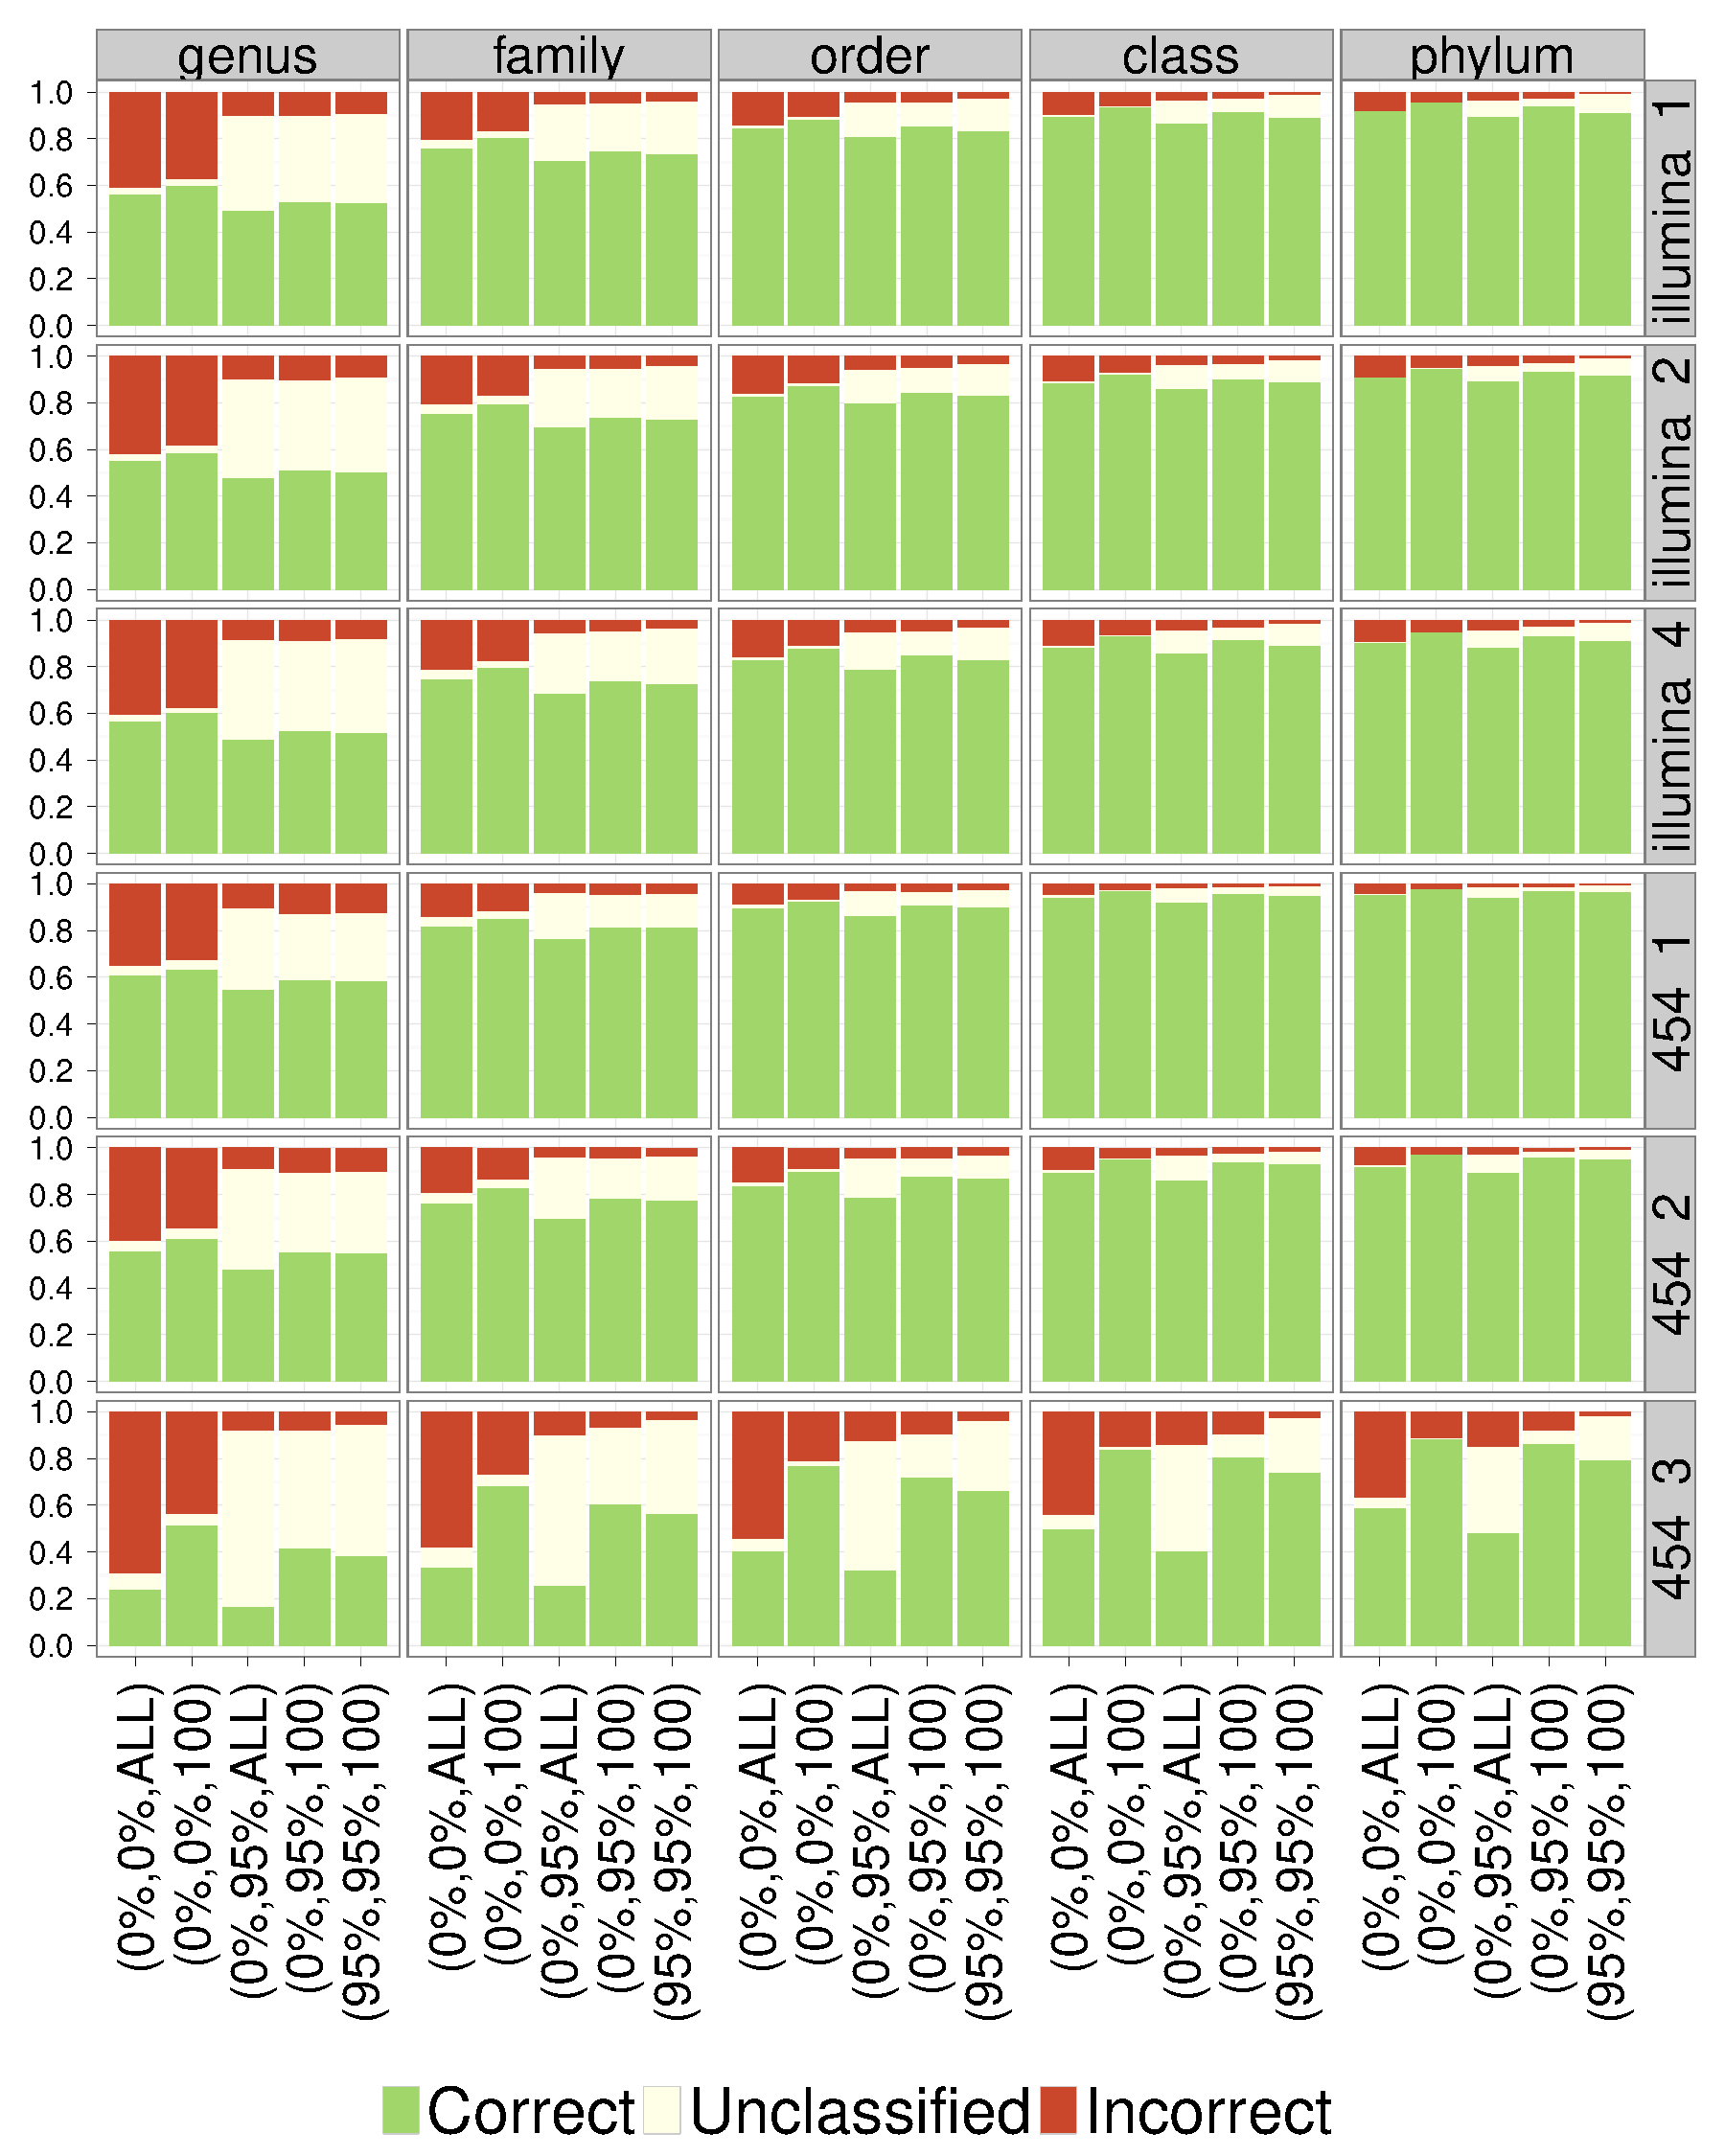
\includegraphics[scale=0.28]{{leaveout/leaveout.higher.species}.pdf}
\end{center}
\caption{\label{tipp:leave_out_tipp_species} Leave-species-out experiment
on the rpsB marker gene, comparing the classification accuracy of different variants of TIPP. 
Each variant is labeled by (X,Y,Z), where X refers to alignment support ($s_a$), Y refers to placement support ($s_p$),
and Z refers to alignment subset size ($m_a$).
Note that SEPP with $m_a=100$
is identical to TIPP(0\%,0\%,100), and that 
HMMER+pplacer is identical to TIPP(0\%,0\%,ALL).}
\end{figure}

\begin{figure}[htpb]
\begin{center}
{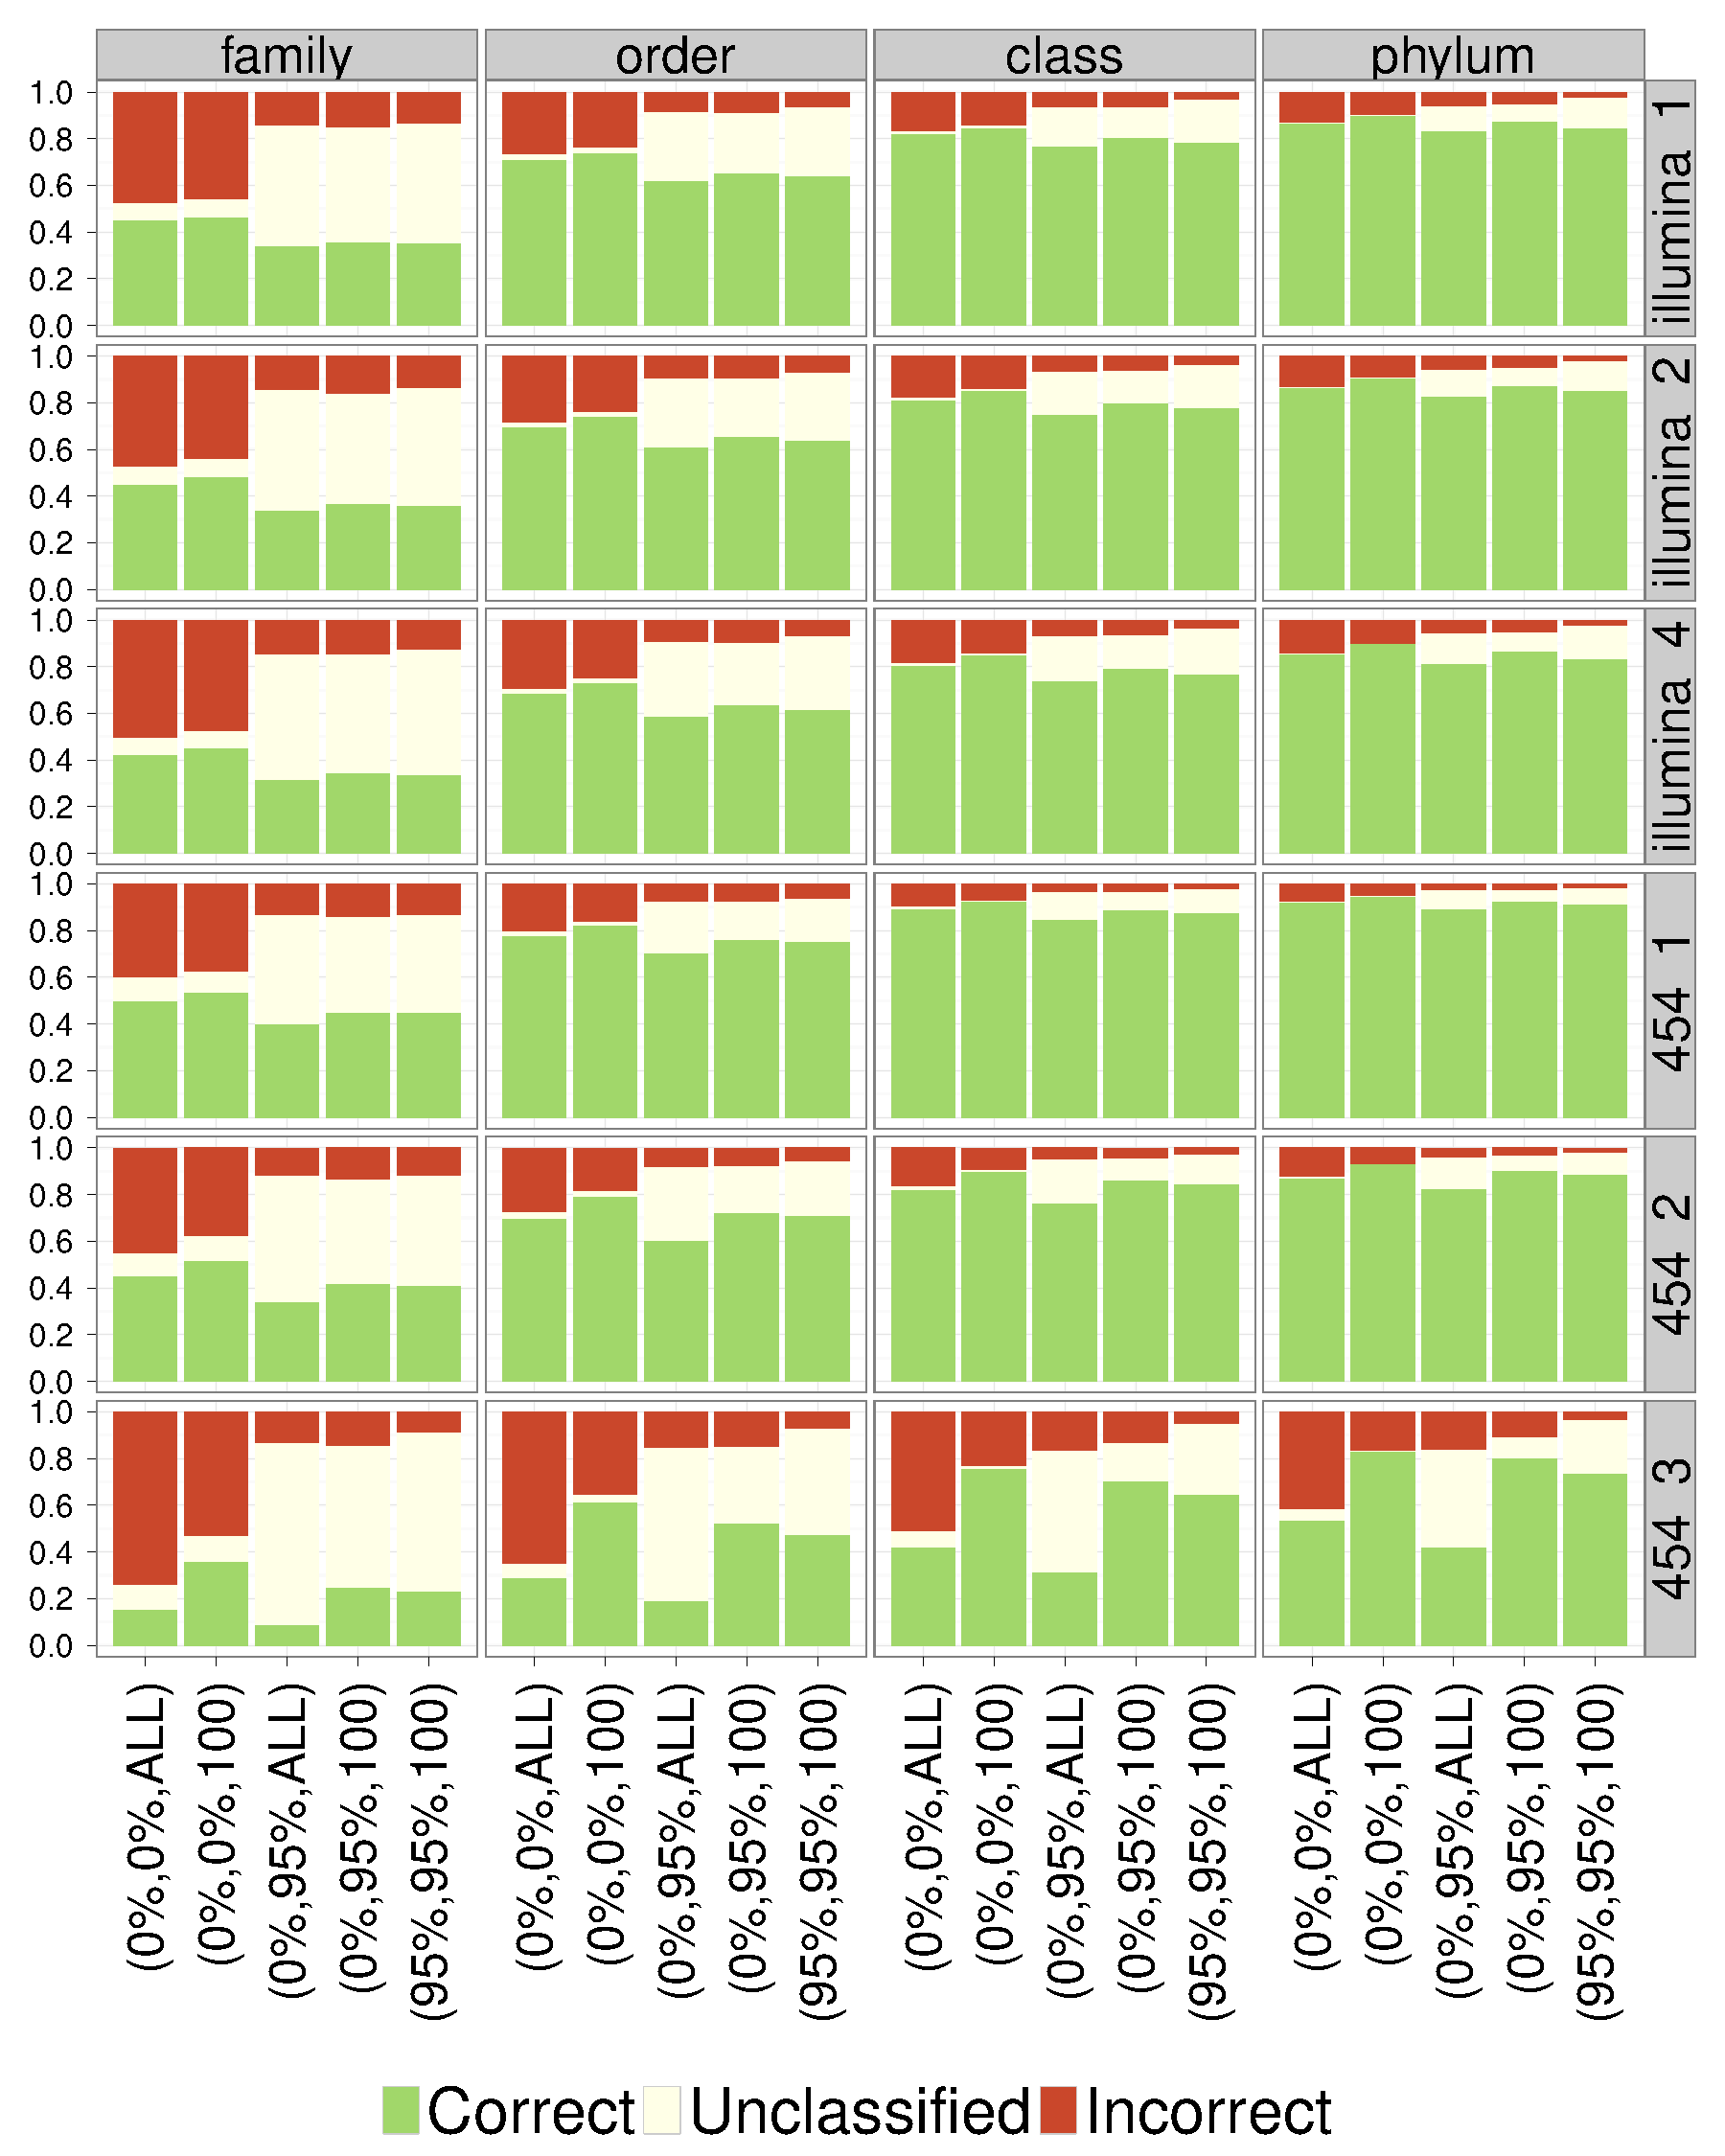
\includegraphics[scale=0.28]{{leaveout/leaveout.higher.genus}.pdf}}
\end{center}
\vspace{-8pt}
\caption{\label{tipp:leave_out_tipp_genus} Leave-genus-out experiment
on the rpsB marker gene,
          comparing the classification accuracy of different variants of TIPP. 
Each variant is labeled by (X,Y,Z), where X refers to alignment support ($s_a$), Y refers to placement support ($s_p$),
and Z refers to alignment subset size ($m_a$). 
%Note that (0\%,0\%,ALL) is equivalent of
%HMMER+pplacer run on the refined taxonomic tree, and (0\%,0\%,100) is equivalent of
%SEPP. (0\%,95\%,ALL) and (0\%,95\%,100) are similar to
%HMMER+pplacer and SEPP, respectively, but consider placement uncertainty. (95\%,95\%,100) corresponds to
%the suggested way of running TIPP (default).
%All results shown here are obtained on rpsB marker gene with both Illumina-like and 454-error like errors.}
%Each column is the classification accuracy
%  for a taxonomic rank and each row the level left out.
%  TIPP($X$\%,$Y$) refers to TIPP run under the default settings with
%  an alignment support and placement support of $X$ and alignment
%  decomposition set size of $Y$.  }
}
\end{figure}

\begin{figure}[htpb]
\begin{center}
{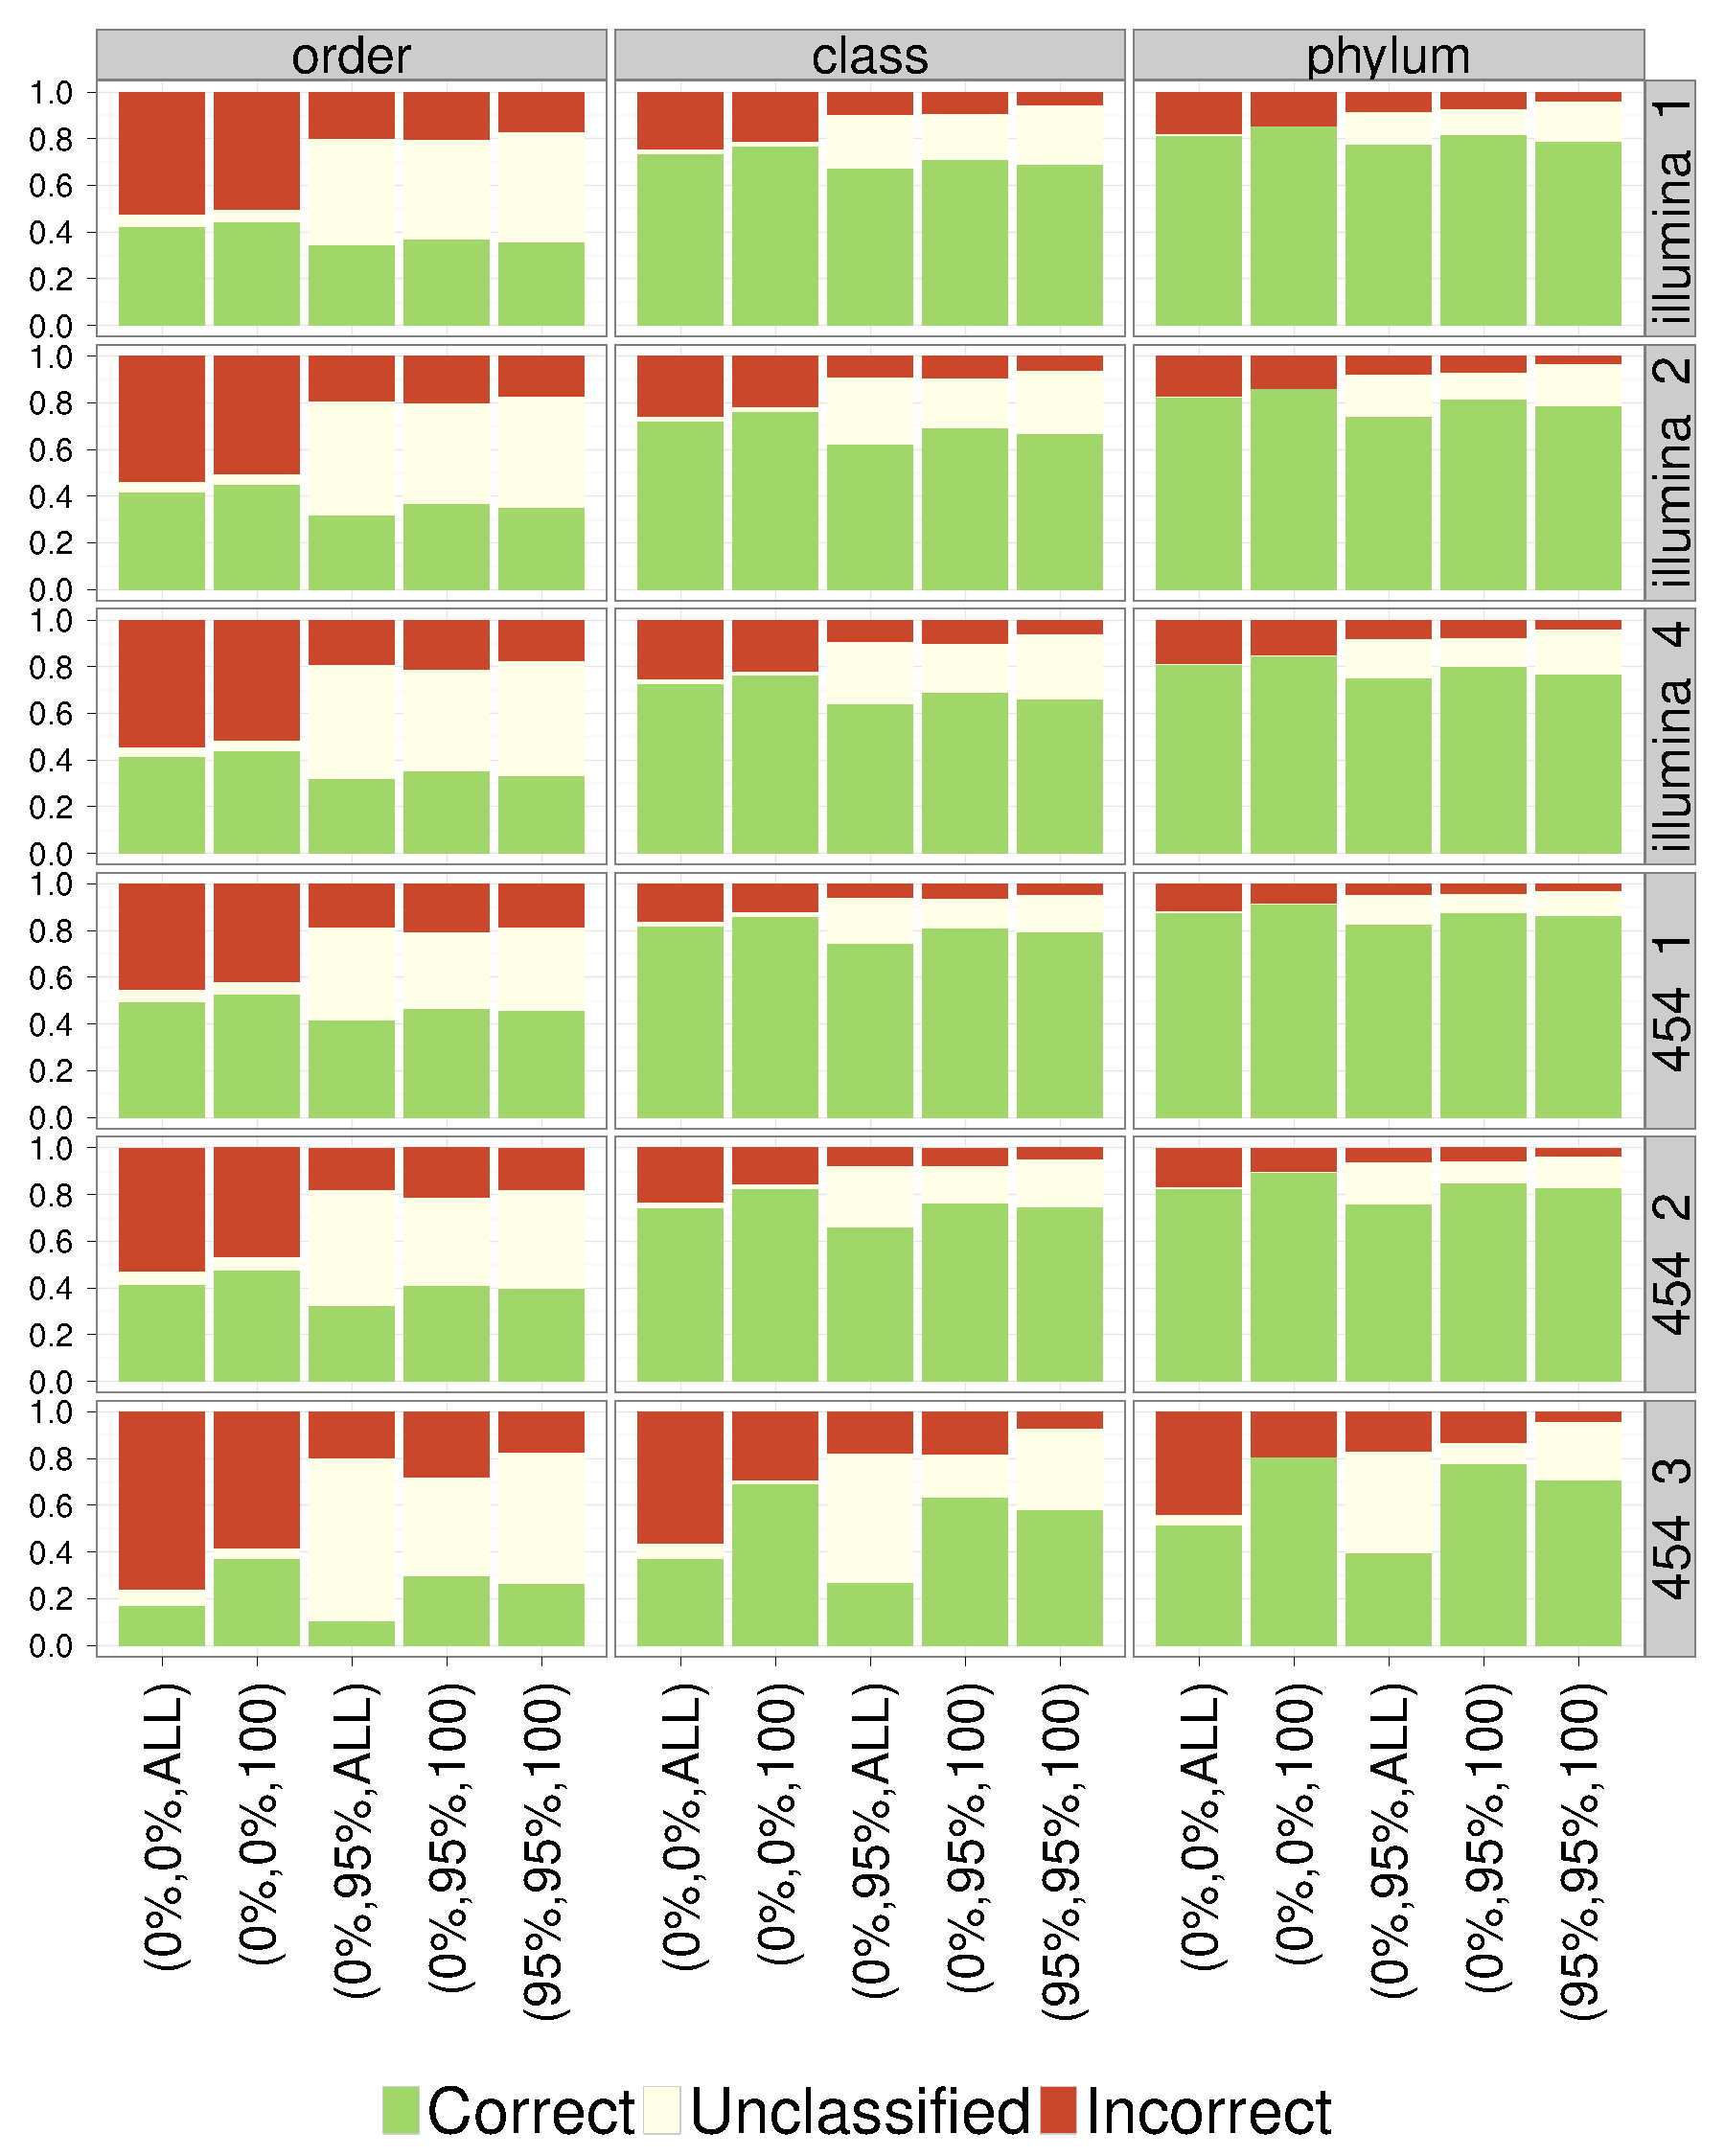
\includegraphics[scale=0.28]{{leaveout/leaveout.higher.family}.pdf}}
\end{center}
\vspace{-8pt}
\caption{\label{tipp:leave_out_tipp_family} Leave-family-out experiment
on the rpsB marker gene,
          comparing the classification accuracy of different variants of TIPP. 
Each variant is labeled by (X,Y,Z), where X refers to alignment support ($s_a$), Y refers to placement support ($s_p$),
and Z refers to alignment subset size ($m_a$). 
%Note that (0\%,0\%,ALL) is equivalent of
%HMMER+pplacer run on the refined taxonomic tree, and (0\%,0\%,100) is equivalent of
%SEPP. (0\%,95\%,ALL) and (0\%,95\%,100) are similar to
%HMMER+pplacer and SEPP, respectively, but consider placement uncertainty. (95\%,95\%,100) corresponds to
%the suggested way of running TIPP (default).
%All results shown here are obtained on rpsB marker gene with both Illumina-like and 454-error like errors.}
%Each column is the classification accuracy
%  for a taxonomic rank and each row the level left out.
%  TIPP($X$\%,$Y$) refers to TIPP run under the default settings with
%  an alignment support and placement support of $X$ and alignment
%  decomposition set size of $Y$.  }
}
\end{figure}
\newpage
% \subsection{Leave-one-out experiments: TIPP versus MetaPhyler}

% In the main paper we showed leave-one-out results comparing TIPP(95\%,95\%,100) and MetaPhyler
% on all marker genes. 
% Here we also show results for TIPP(50\%,50\%,100) in the same experimental setting. 
% Figures \ref{tipp:leave_out_16_bacteria_i} to \ref{tipp:leave_out_30M_i} show results
% similar to Experiment 3 of the main paper, with the addition of TIPP(50\%,50\%,100).

% By design, 
% TIPP(50\%,50\%,100) has higher classification rates than TIPP(95\%,95\%,100), but also has a higher false positive.
% In situations where the reference tree is unlikely to include all bacteria in the community,
% and when revealing new species is important, using more stringent settings is therefore suggested.

% \begin{figure}[htpb]
% \begin{center}
% \subfigure[16S bacteria; Illumina error\label{tipp:leave_out_16_bacteria_i}]{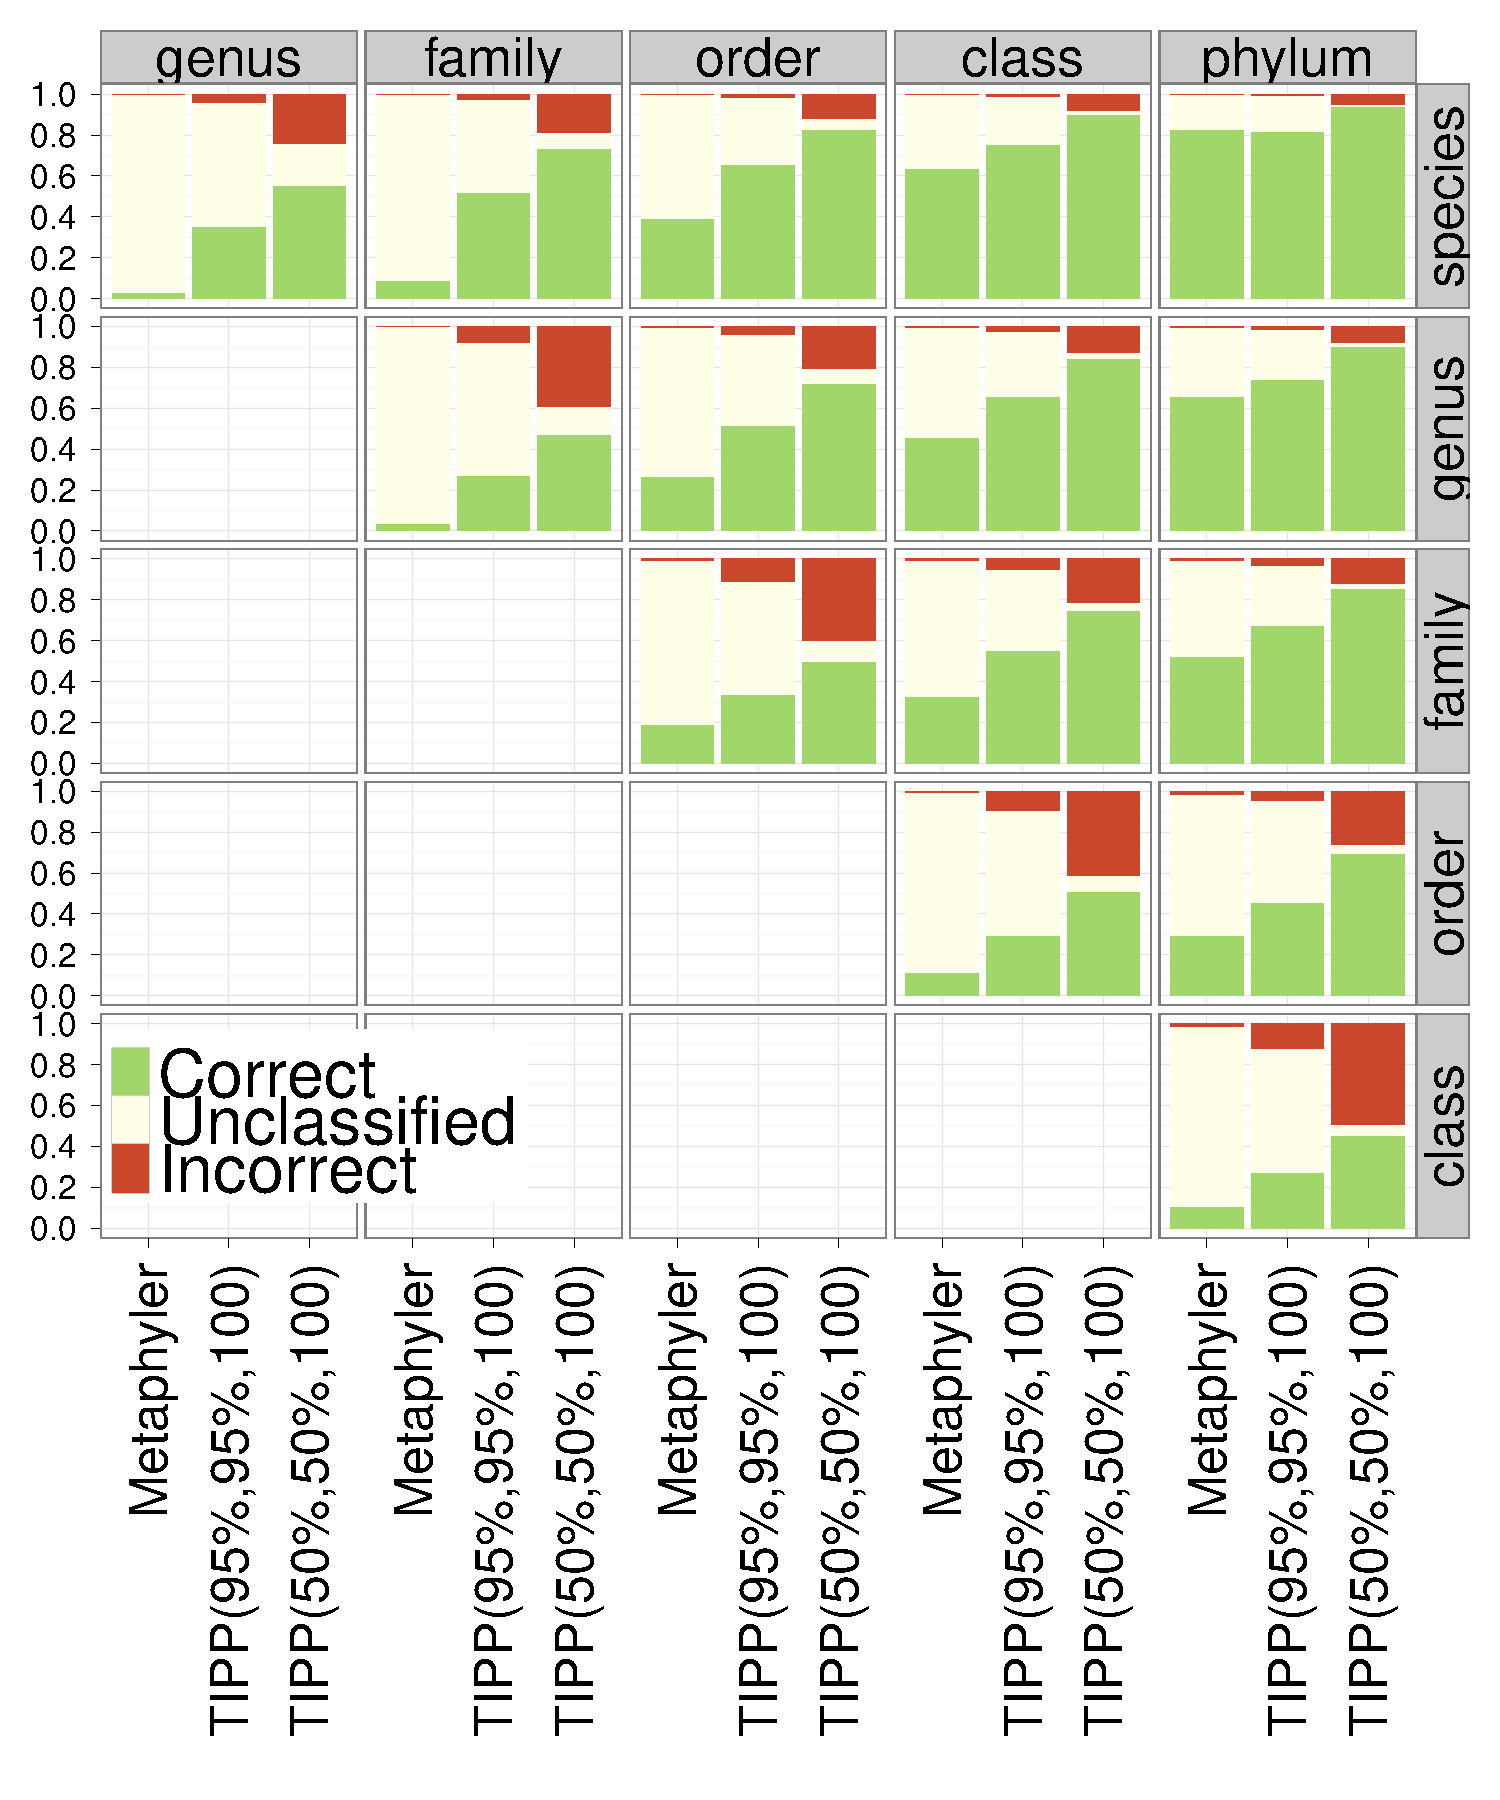
\includegraphics[scale=0.320]{{leaveout/leaveout.illumina.old.16S_bacteria}.pdf}}
% \subfigure[16S bacteria; 454 error\label{tipp:leave_out_16_bacteria_4}]{\includegraphics[scale=0.320]{{leaveout/leaveout.454.old.16S_bacteria}.pdf}}
% \end{center}
% \caption{\label{tipp:leave_out_16-Bacteria} Leave-one-out experiment
          % comparing MetaPhyler
          % to TIPP on the bacterial dataset using the 16S RNA gene,
          % with both Illumina-like and 454-like error models.
	  % For the analyses of the bacterial dataset, due to computational challenges, 
% the placement size is set to 1,000, and the taxonomic tree is used for alignment decomposition.}

% Each column is the classification accuracy
 % for a taxonomic rank and each row the level left out.
 % TIPP($X$\%,$Y$) refers to TIPP run under the default settings with
 % an alignment support and placement support of $X$ and alignment
 % decomposition set size of $Y$.  }
% \end{figure}

% \begin{figure}[htpb]
% \begin{center}
% \subfigure[16S archaea; Illumina error\label{tipp:leave_out_16_archaea_i}]{\includegraphics[scale=0.32]{{leaveout/leaveout.illumina.old.16S_archaea}.pdf}}
% \subfigure[16S archaea; 454 error\label{tipp:leave_out_16_archaea_4}]{\includegraphics[scale=0.32]{{leaveout/leaveout.454.old.16S_archaea}.pdf}}
% \end{center}
% \caption{\label{tipp:leave_out_16-Archaea} Leave-one-out experiment
          % comparing MetaPhyler
          % to TIPP on the archae dataset using the 16S  gene,
          % with both Illumina-like and 454-like error models.
     % }

% Each column is the classification accuracy
 % for a taxonomic rank and each row the level left out.
 % TIPP($X$\%,$Y$) refers to TIPP run under the default settings with
 % an alignment support and placement support of $X$ and alignment
 % decomposition set size of $Y$.  }
% \end{figure}

% \begin{figure}[htpb]
% \begin{center}

% \subfigure[Illumina error model\label{tipp:leave_out_30M_i}]{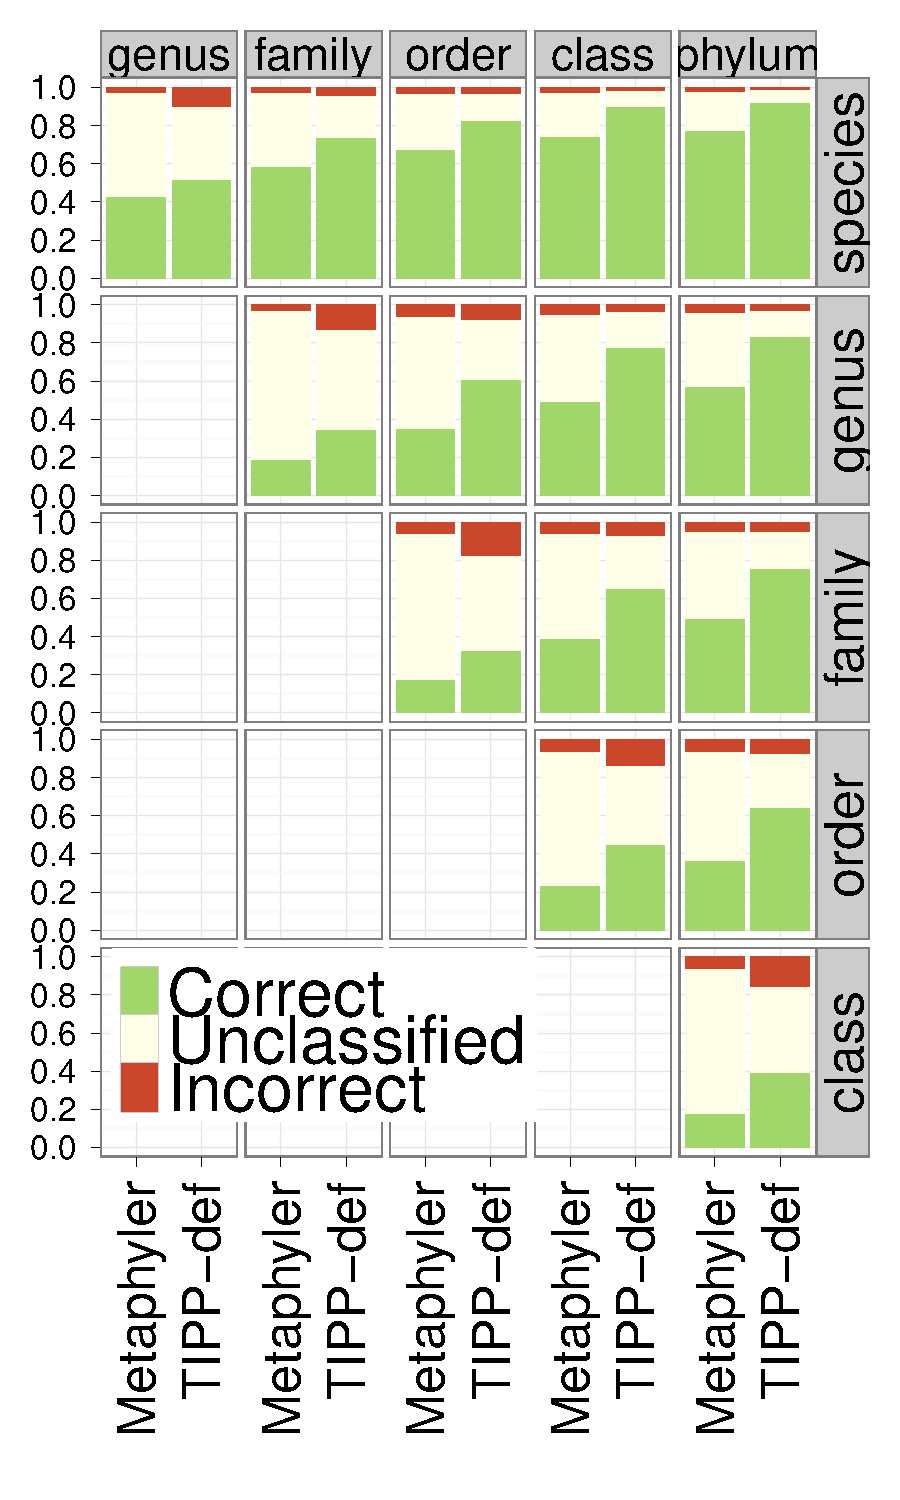
\includegraphics[scale=0.32]{{leaveout/leaveout.illumina.old}.pdf}}
% \subfigure[454 error model\label{tipp:leave_out_30M_4}]{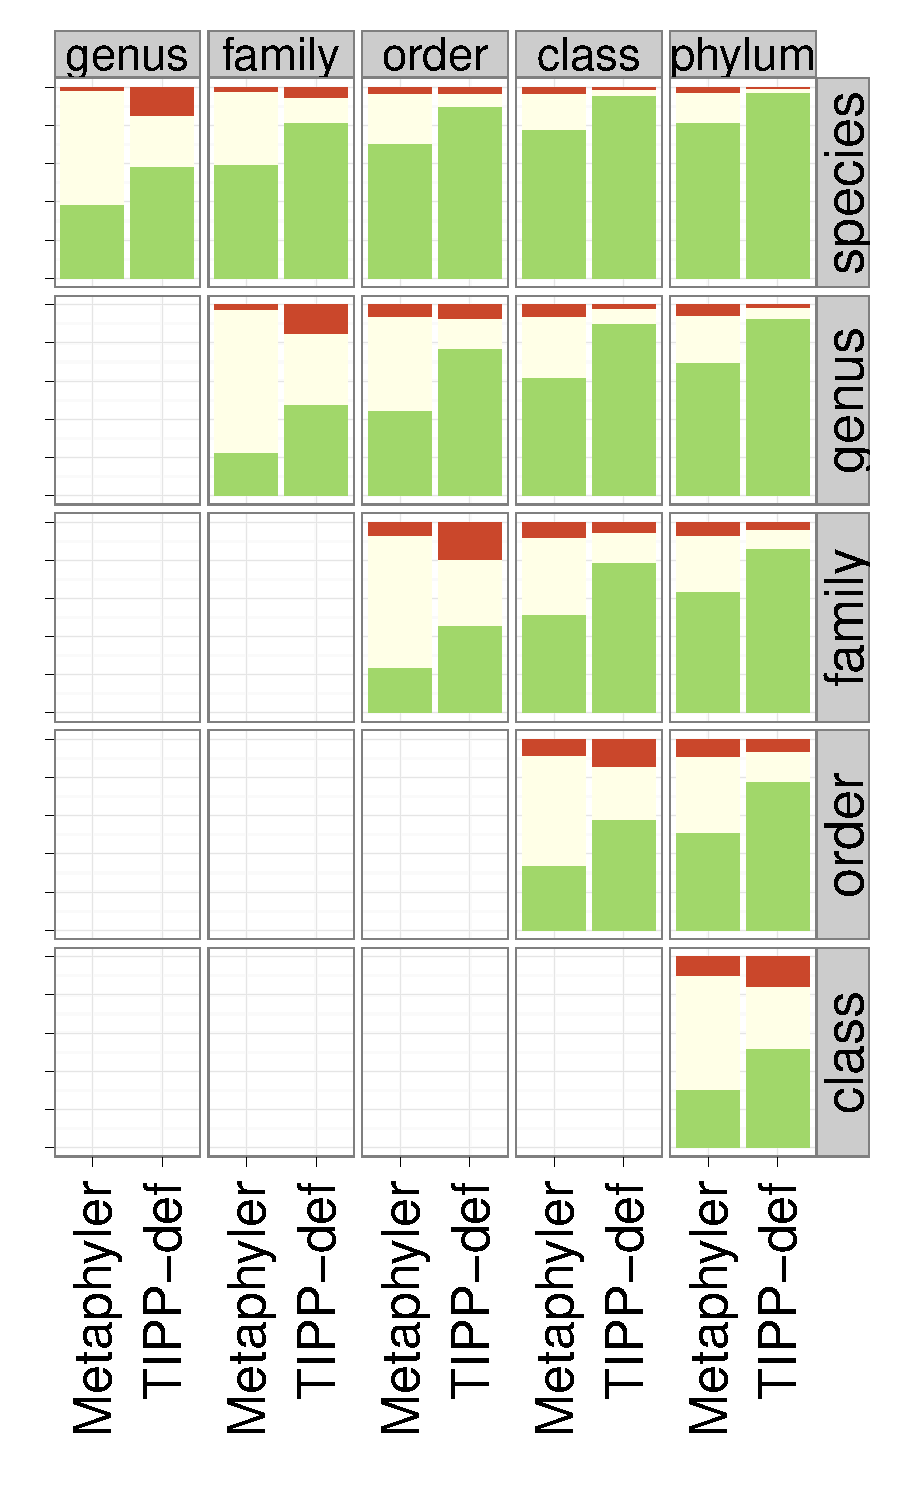
\includegraphics[scale=0.32]{{leaveout/leaveout.454.old}.pdf}}
% \end{center}
% \caption{\label{tipp:leave_out_30M} Leave-one-out experiment
          % comparing the classification accuracy for MetaPhyler
          % versus TIPP on 30 marker genes with both Illumina-like and 454-error like errors.  
% }
% Each column is the classification accuracy
 % for a taxonomic rank and each row the level left out.
 % TIPP($X$\%,$Y$) refers to TIPP run under the default settings with
 % an alignment support and placement support of $X$ and alignment
 % decomposition set size of $Y$.  }
% \end{figure}

\newpage
\subsection{TIPP Boosting of EPA versus pplacer}\label{tipp:tipp.epa.pplacer.sec}
TIPP requires an external placement tool for its placement step. 
While the initial submission only used pplacer, the current
current implementation of TIPP
can use both pplacer and EPA. The results in the main
paper are based on using pplacer internally, and here we 
show results on using EPA inside TIPP, compared 
to using pplacer inside TIPP, in a leave-species-out experiment on the rpsB marker gene. 
We observe that in this experiment, TIPP using pplacer and EPA 
are almost identical
(Figure \ref{tipp:tipp.epa.pplacer});
the differences in recall between 
the two techniques are statistically
significant only when placing at the class or phylum level and
the differences between precision is never statistically significant (Table \ref{tipp:tipp.epa.pplacer.tab}). 

\begin{figure}[htpb]
\begin{center}
\includegraphics[scale=0.32]{{leaveout/leaveout.epa_pplacer.species}.pdf}
\end{center}
\caption{\label{tipp:tipp.epa.pplacer} Leave-one-out experiment
          comparing the classification accuracy for TIPP with default settings when it uses EPA or pplacer internally
for the placement step. Results are for a leave-species-out experiment on the rpsB marker 
gene with Illumina-like errors. Differences in recall are
statistically significant at the class and phylum levels, but not
below the class level.   }
\end{figure}

\begin{table}[hptb]
\caption{\label{tipp:tipp.epa.pplacer.tab} Precision and recall of TIPP when it uses EPA or pplacer internally
for the placement step. The table shows the difference between precision and recall 
values of the two techniques (delta) and p-value of a statistical test showing
whether the differences are statistically significant according to the Pearson's chi-square contingency table test (as implemented in R~\cite{R}).
Positive values mean TIPP with pplacer was better than TIPP with EPA.
Results are for a leave-species-out experiment on the rpsB marker 
gene with Illumina-like errors. 
Differences in recall are
statistically significant at the class and phylum levels, but not
below the class level. In all other cases differences are not statistically significant. }
\begin{center}
\begin{tabular}{|l|c|c|c|c|c|} \hline
&\multicolumn{1}{|c|}{genus}&\multicolumn{1}{c|}{family}&\multicolumn{1}{c|}{order}&\multicolumn{1}{c|}{class}&\multicolumn{1}{c|}{phylum}\\ \hline
{\bf Recall} &&&&&\\
~Delta &~0.006&~0.012&~0.013&{\bf ~0.013}&{\bf ~0.011}\\ 
~p-value &0.5617&0.1975&0.0763&{\bf 0.0244}&{\bf 0.0165}\\ \hline
{\bf Precision} &&&&&\\
~Delta &~0.000&-0.001&~0.002&~0.003&~0.001\\ 
~p-value & 0.9960&0.8662&0.6282&0.2412&0.4704\\ 
\hline
\end{tabular}
\end{center}
\end{table}

\newpage
\subsection{Non-leave-one-out Parameter Exploration Study}\label{supp:tipp_non_leaveout_variants}
In this section we report on non-leave-one-out experiments performed on the rpsB marker gene
in order to further understand the impact of parameter settings on the accuracy of TIPP. Note that results from
these non-leave-one-out experiments should be interpreted in conjunction with
leave-one-out results presented earlier. The impact of parameter settings could
be quite different between non-leave-one-out and leave-one-out results, hence caution is required in interpreting the results. 
In general, changing TIPP parameters show a higher impact on classification accuracy in leave-one-out experiments. 
In non-leave-one-out experiments, the impact of
changes to the TIPP parameters is often most observable at the highest error model conditions.

\paragraph{Placement Support.}  Placement support has a large impact on the overall classification accuracy (Fig.~\ref{tipp:placement_support}). For both types of sequencing error, the largest of varying placement support is at the species level; increasing the placement support results in fewer incorrect and correct classifications.  The impact of placement support is most visible on 454 models with higher rates of error.  A sizeable portion of the false positives can be removed by using higher placement support values.

\begin{figure}[htpb]
\begin{center}
\begin{subfigure}[htpb]{\textwidth}
\includegraphics[scale=0.300]{{higher_error/higher_error_illumina_placement_1_5_13}.pdf}\\
\caption[]{Illumina-like fragments}
\end{subfigure}
\end{center}
\begin{center}
\begin{subfigure}[htpb]{\textwidth}
\includegraphics[scale=0.300]{{higher_error/higher_error_454_placement_1_5_13}.pdf}\\
\caption[]{454-like fragments}
\end{subfigure}
\end{center}
\caption[Varying placement support.]{\label{tipp:placement_support}Non-leave-one-out experiments showing the impact of changing placement support on the classification accuracy for fragments simulated from the rpsB gene with (a) Illumina-like errors and (b) 454-error like errors.  Each column is the classification accuracy for a taxonomic rank and each row is the error model used.  TIPP($X$\%,$Y$\%,$Z$) refers to TIPP run under the default settings with an alignment support of $X$, placement support of $Y$, and maximum alignment decomposition subset size of $Z$.}
\end{figure}

\paragraph{Alignment Support.}  Figures~\ref{tipp:alignment_support_50} and ~\ref{tipp:alignment_support_95} show the result of fixing the placement support to be 50\% or 95\%, and changing the alignment support threshold.  Increasing the alignment support has a slight impact on the overall classification accuracy for the Illumina-type errors.  The differences between the percentage of fragments classified at all levels for 0\% alignment support and 95\% alignment support is less than 5 percentage points. 
For the 454-type errors, the impact of alignment support is only noticeable for the higher error model conditions.  
Note that leave-one-out results were impacted more by varying alignment support.

\begin{figure}[htpb]
\begin{center}
\begin{subfigure}[htpb]{\textwidth}
\includegraphics[scale=0.300]{{higher_error/higher_error_illumina_alignment_50_1_5_13}}\\
\caption[]{Illumina-like fragments}
\end{subfigure}
\end{center}
\begin{center}
\begin{subfigure}[htpb]{\textwidth}
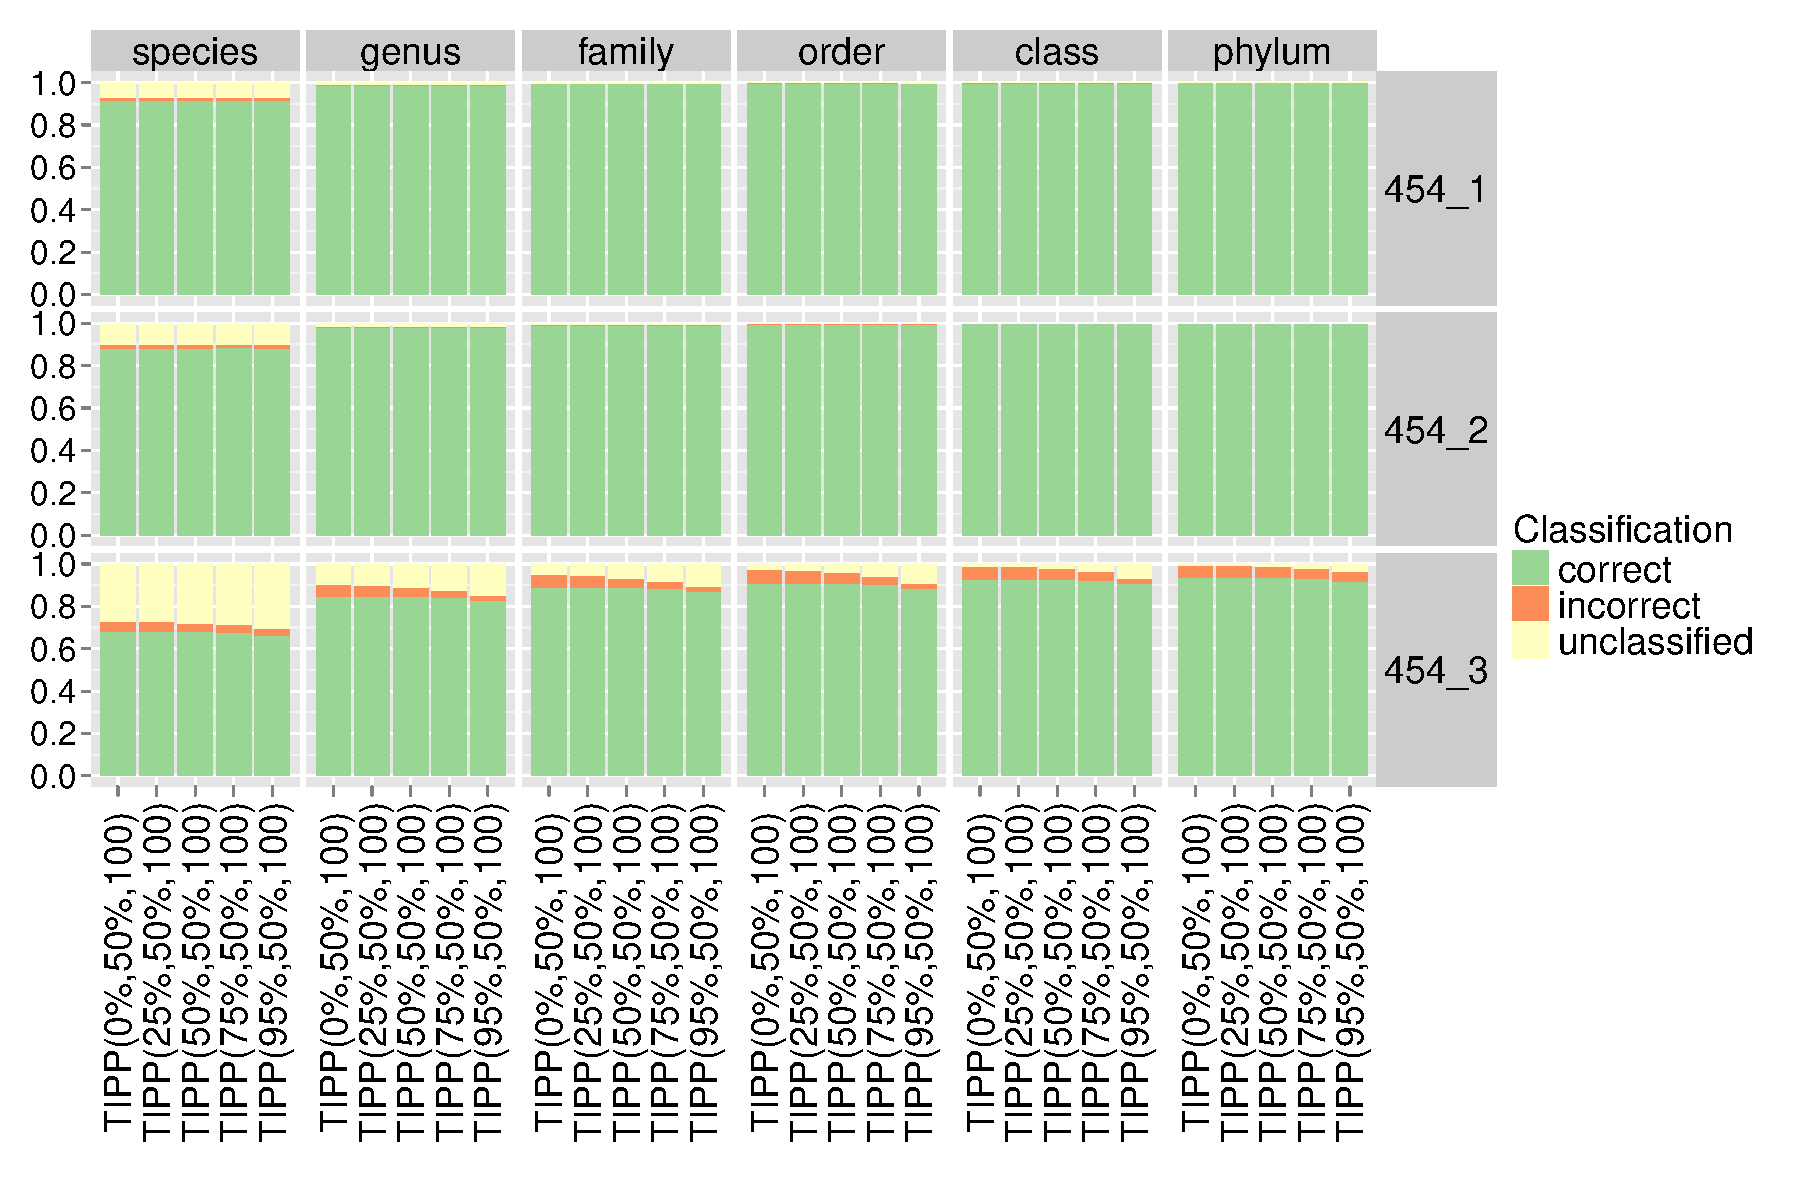
\includegraphics[scale=0.300]{{higher_error/higher_error_454_alignment_50_1_5_13}}\\
\caption[]{454-like fragments}
\end{subfigure}
\end{center}
\caption[Varying alignment support with placement support of 50\%.]{\label{tipp:alignment_support_50}Non-leave-one-out experiments showing the impact of changing alignment support while fixing the placement support to be 50\% on the classification accuracy for fragments simulated under the (a) Illumina error model and (b) 454 error model for the rpsB marker gene.  Each column is the classification accuracy for a taxonomic rank and each row is the error model used.  TIPP($X$\%,$Y$\%,$Z$) refers to TIPP run under the default settings with an alignment support of $X$, placement support of $Y$, and maximum alignment decomposition subset size of $Z$.}
\end{figure}

\begin{figure}[htpb]
\begin{center}
\begin{subfigure}[htpb]{\textwidth}
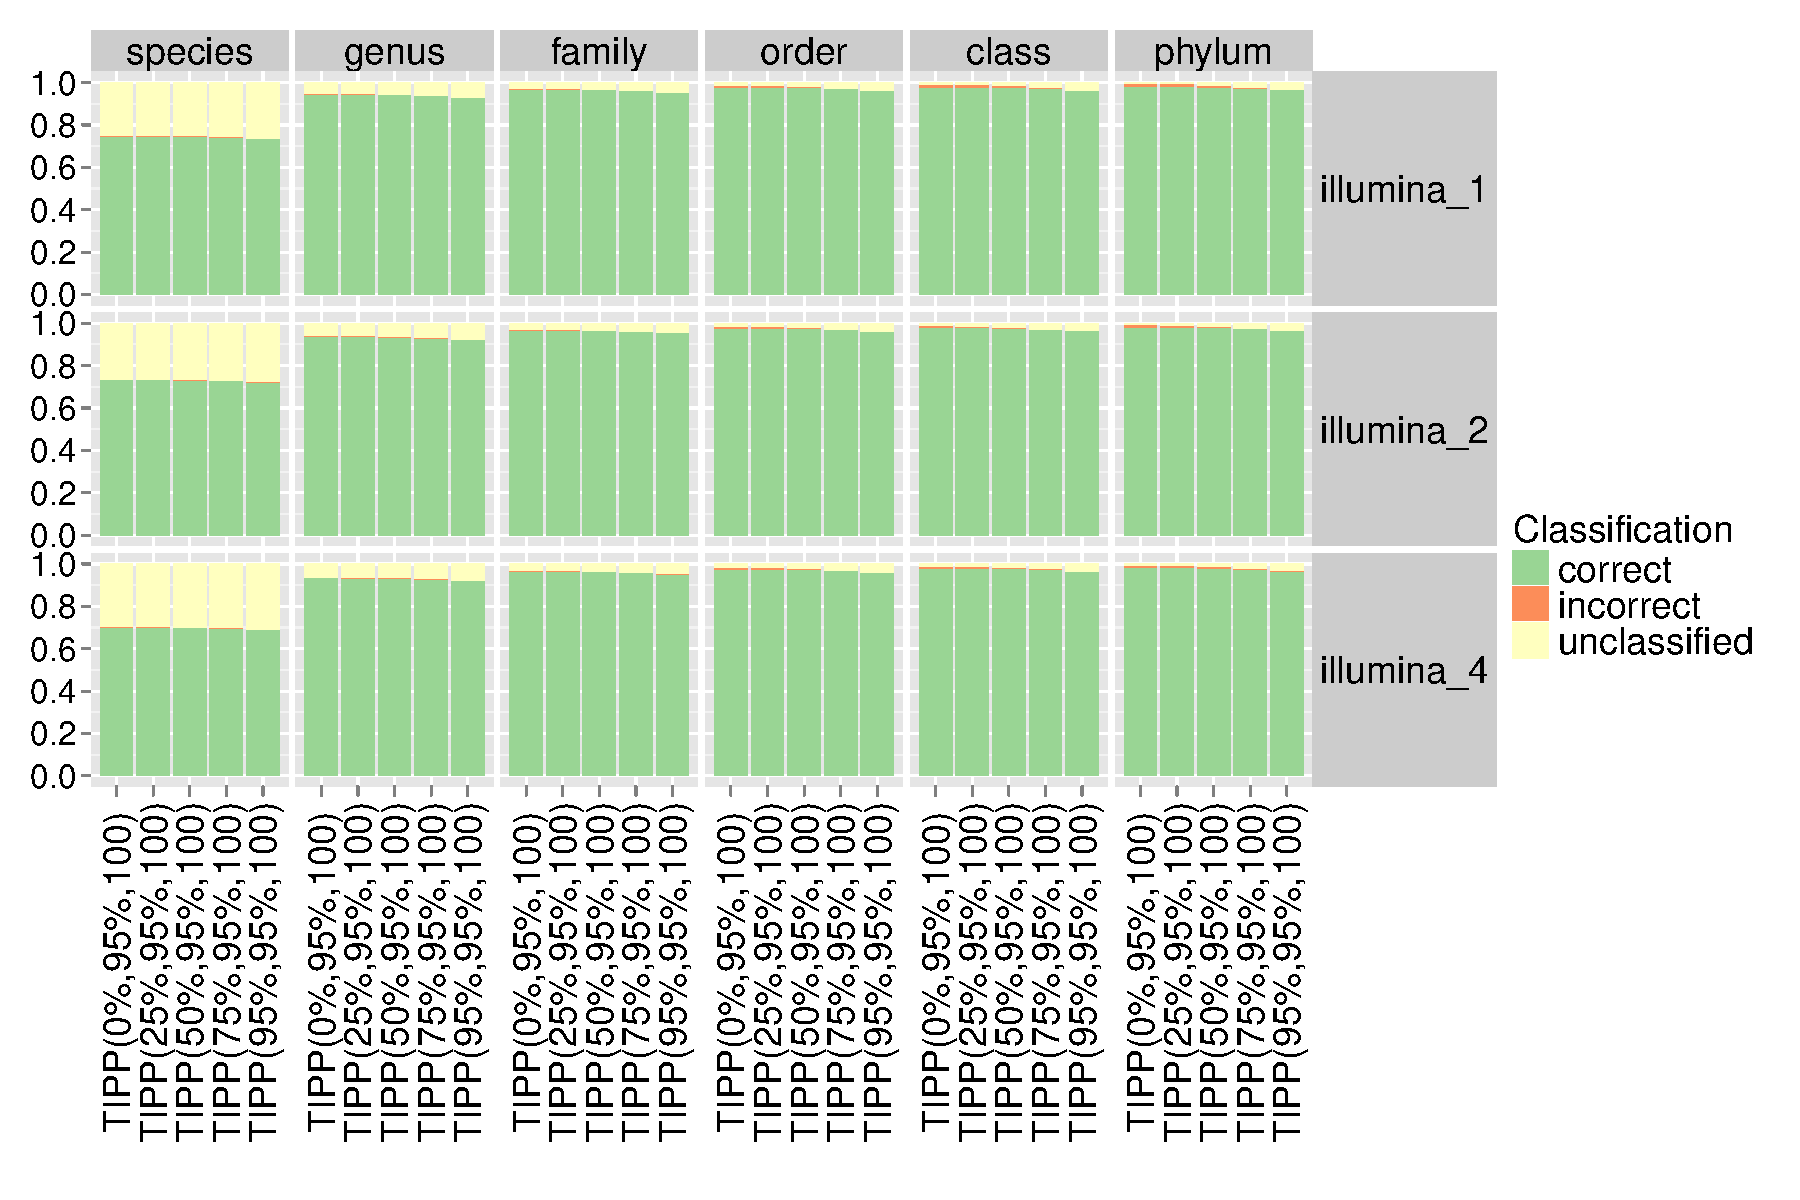
\includegraphics[scale=0.300]{{higher_error/higher_error_illumina_alignment_95_1_5_13}}\\
\caption[]{Illumina-like fragments}
\end{subfigure}
\end{center}
\begin{center}
\begin{subfigure}[htpb]{\textwidth}
\includegraphics[scale=0.300]{{higher_error/higher_error_454_alignment_95_1_5_13}}\\
\caption[]{454-like fragments}
\end{subfigure}
\end{center}
\caption[Varying alignment support with placement support of 95\%.]{\label{tipp:alignment_support_95}Non-leave-one-out experiments showing the impact of changing alignment support while fixing the placement support to be 95\% on the classification accuracy for fragments simulated under the (a) Illumina error model and (b) 454 error model for the rpsB marker gene.  Each column is the classification accuracy for a taxonomic rank and each row is the error model used.  TIPP($X$\%,$Y$\%,$Z$) refers to TIPP run under the default settings with an alignment support of $X$, placement support of $Y$, and maximum alignment decomposition subset size of $Z$.}
\end{figure}

\paragraph{Alignment Support and Placement Support.} Figure~\ref{tipp:general_support} shows the result of changing alignment support and placement support together.  TIPP(0\%,0\%,100) tends to over-classify, resulting in the largest percentage of  incorrect classifications.  Both TIPP(25\%,25\%,100) and TIPP(50\%,50\%,100) result in a drop of correct classifications at the species level, but, at the same time, a larger drop in incorrect classifications at the species level.  The drop in correct classifications is not noticeable for the higher taxonomic levels on the error models with low rates of error.   TIPP(95\%,95\%,100) has a large decrease of correct classifications at the species level, but also has the fewest incorrect classifications at all levels for all error models; nearly all the error for the lower error model conditions are eliminated.
%From result, propose two versions of TIPP, TIPP liberal (TIPP(50\%,50\%)) and conservative version (TIPP(95\%,95\%)).  
%\textbf{Need to justify why 50\% and why 95\%}
%\textbf{ADD ROC CURVES FOR RESULTS}

\begin{figure}[htpb]
\begin{center}
\begin{subfigure}[htpb]{\textwidth}
\includegraphics[scale=0.300]{{higher_error/higher_error_illumina_best_1_5_13}}\\
\caption[]{Illumina-like fragments}
\end{subfigure}
\end{center}
\begin{center}
\begin{subfigure}[htpb]{\textwidth}
\includegraphics[scale=0.300]{{higher_error/higher_error_454_best_1_5_13}}\\
\caption[]{454-like fragments}
\end{subfigure}
\end{center}
\caption[Varying alignment support and placement support.]{\label{tipp:general_support}Non-leave-one-out experiments showing the impact of changing both alignment support and placement support on classification accuracy for fragments simulated from the rpsB gene with (a) Illumina-like errors and (b) 454-error like errors.  Each column is the classification accuracy for a taxonomic rank and each row is the error model used.  TIPP($X$\%,$Y$\%,$Z$) refers to TIPP run under the default settings with an alignment support of $X$, placement support of $Y$, and maximum alignment decomposition subset size of $Z$.
}
\end{figure}


\paragraph{Impact of maximum alignment subset size. }
We found that using smaller alignment subset sizes tends to improve accuracy, 
especially at the species level,
but also increases the running time as there are more alignment subsets to analyze:
the wall clock time to classify 200,000 fragments from the rpsB gene ranged from 2.1 hours  for TIPP(95\%,95\%,ALL) to 3.6 hours for TIPP-default (TIPP(95\%,95\%,100)) (each run with 4 CPUs).  The number of sequences in the reference alignment also impacts the running time for the TIPP(95\%,95\%,ALL) method, but this scales (at most) linearly with the number of sequences. The running time shown for the rpsB gene is a good case study, since the reference alignment has 1463 sequences and is one of the larger datasets  in this study.

Figure ~\ref{tipp:alignment_size_95} shows the impact of changing the alignment decomposition size on TIPP(95\%,95\%).  The result shows that, in general, decreasing the alignment decomposition size increases the percentage of correctly classified fragments, as well as decreases the percentage of incorrectly classified fragments.  
In other words, smaller alignment subsets produce more accurate placements.
However, using smaller alignment decomposition sizes results in an increase in running time.

\begin{figure}[htpb]
\begin{center}
%\subfigure[Illumina-like fragments]{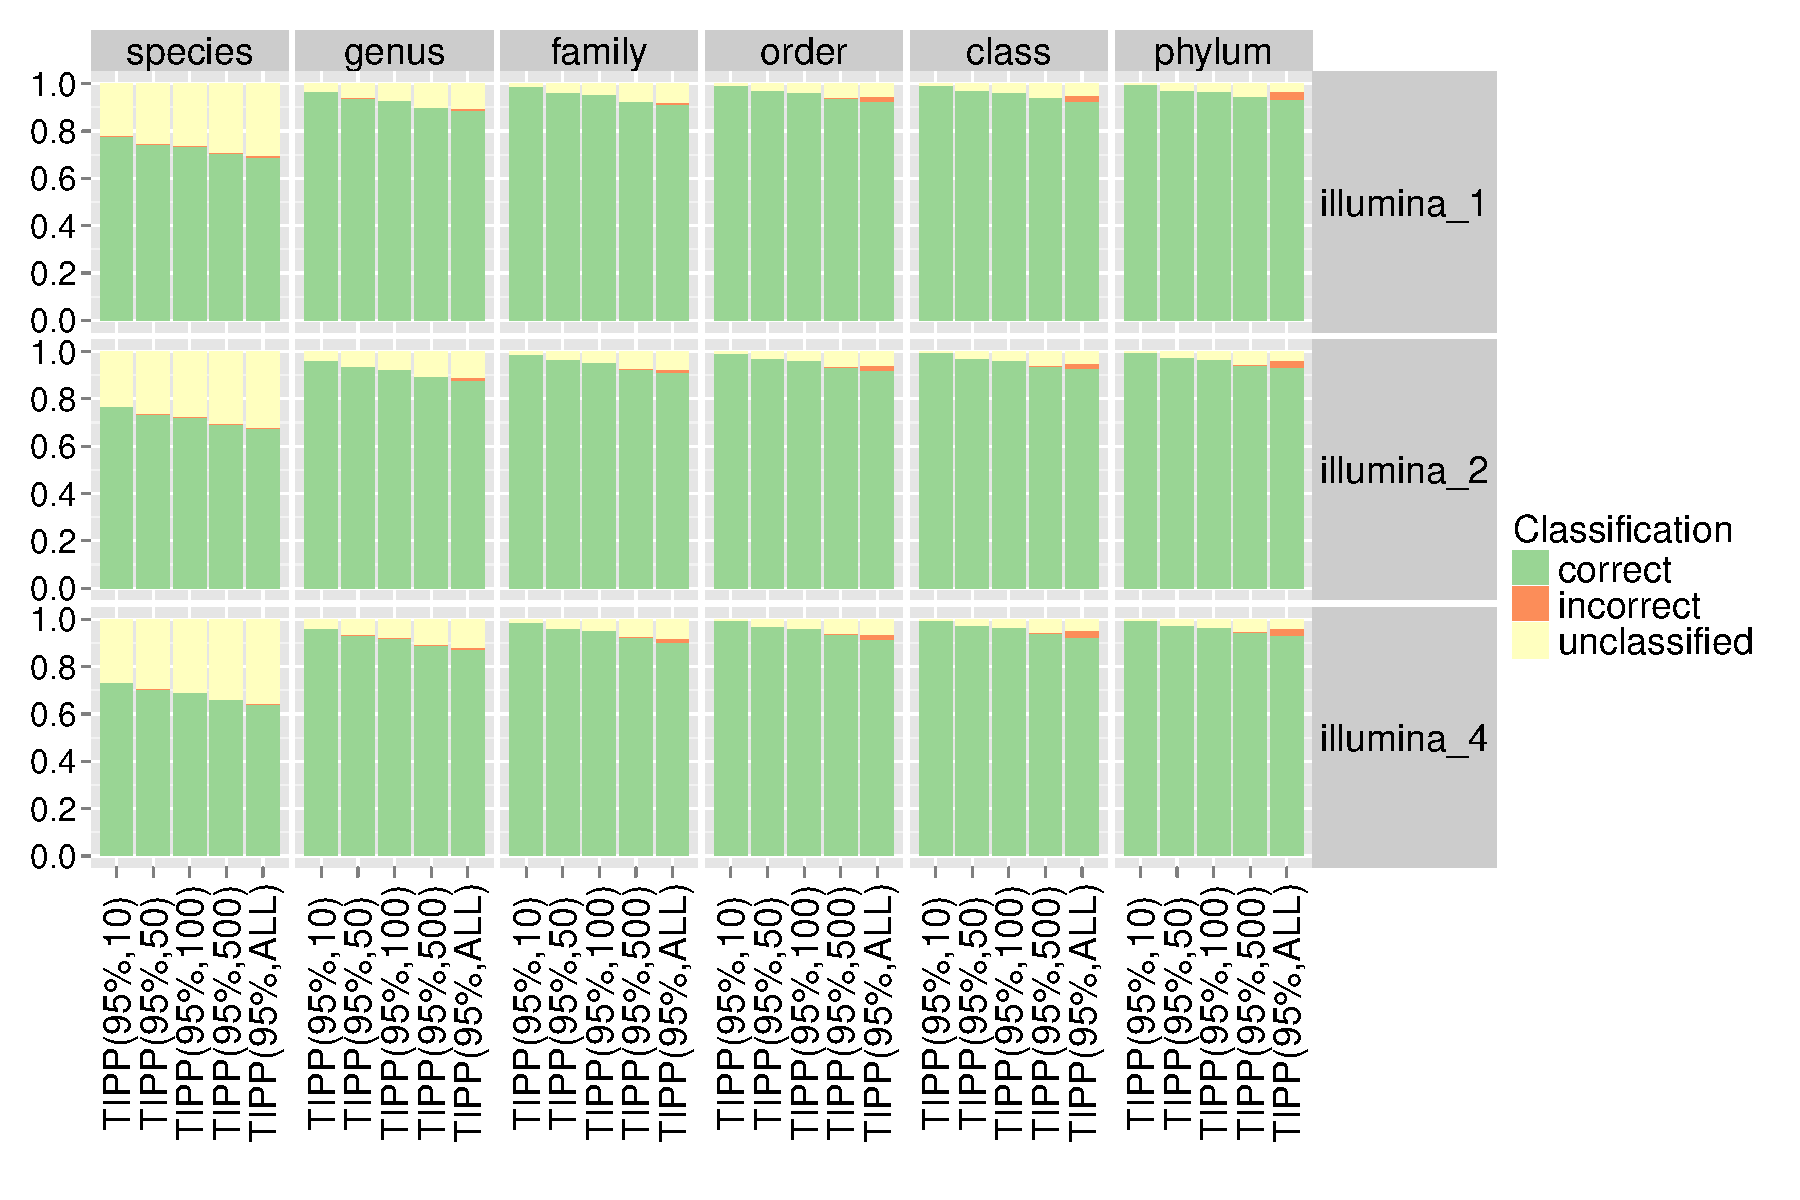
\includegraphics[scale=0.300]{higher_error/higher_error_illumina_size_95_1_5_13}}\\
\end{center}
\begin{center}
%\subfigure[454-like fragments]{\includegraphics[scale=0.300]{higher_error/higher_error_454_size_95_1_5_13}}\\
\end{center}
\caption[Varying decomposition size for TIPP(95\%).]{\label{tipp:alignment_size_95}Non-leave-one-out experiments showing the impact of changing the size of the alignment decomposition for TIPP(95\%) for fragments simulated from the rpsB gene with (a) Illumina-like errors and (b) 454-error like errors.  Each column is the classification accuracy for a taxonomic rank and each row is the error model used. TIPP($X$\%,$Y$) refers to TIPP run under the default settings with an alignment support and placement support of $X$ and a maximum alignment decomposition subset size of $Y$.
}
\end{figure}


\subsection{ROC Curves}
Here we explore the impact of change in support threshold for
alignment subsets of size $10$ in a non-leave-one-out experiment on
the rpsB marker gene (one of the hardest in the dataset), as
alignment and placement support thresholds are increased progressively.

The ROC curves shown in Figure \ref{tipp:roc_curve_full} show
that the impact of the support thresholds
is very visible at the species level, very reduced at the genus level, and then largely
eliminated at the family level and above.  
The curves for the species-level classification show that there is a tight
 relationship between the precision and recall as the
support varies between 0\% to 50\%, but that
the gain in precision
moving from 50\% support to 95\% support is significantly smaller than
the loss in recall (1-2\% gain in precision but 6-10\% drop in
recall).  

\begin{figure}[htpb]
\begin{center}
%\subfigure[Results on rpsB data, non-leave-one-out]{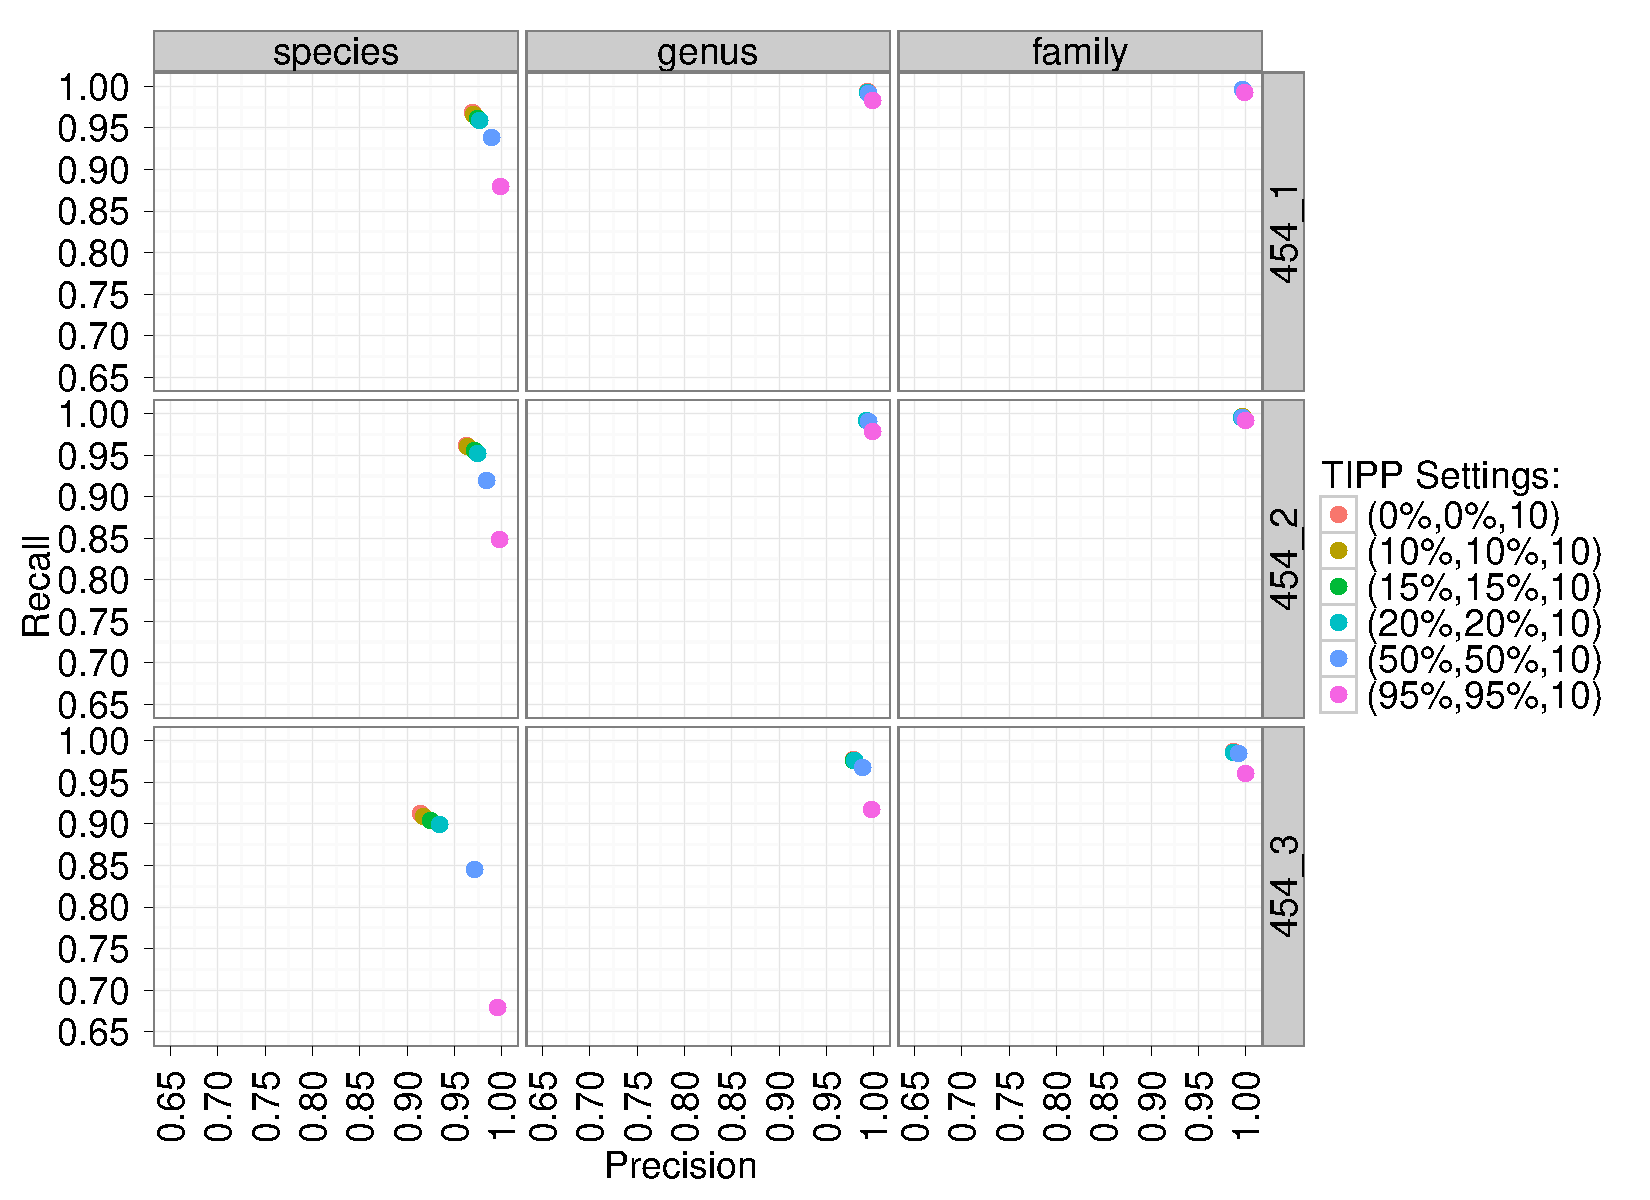
\includegraphics[scale=0.250]{higher_error/roc_higher_error_illumina_all_1_5_12}}\\
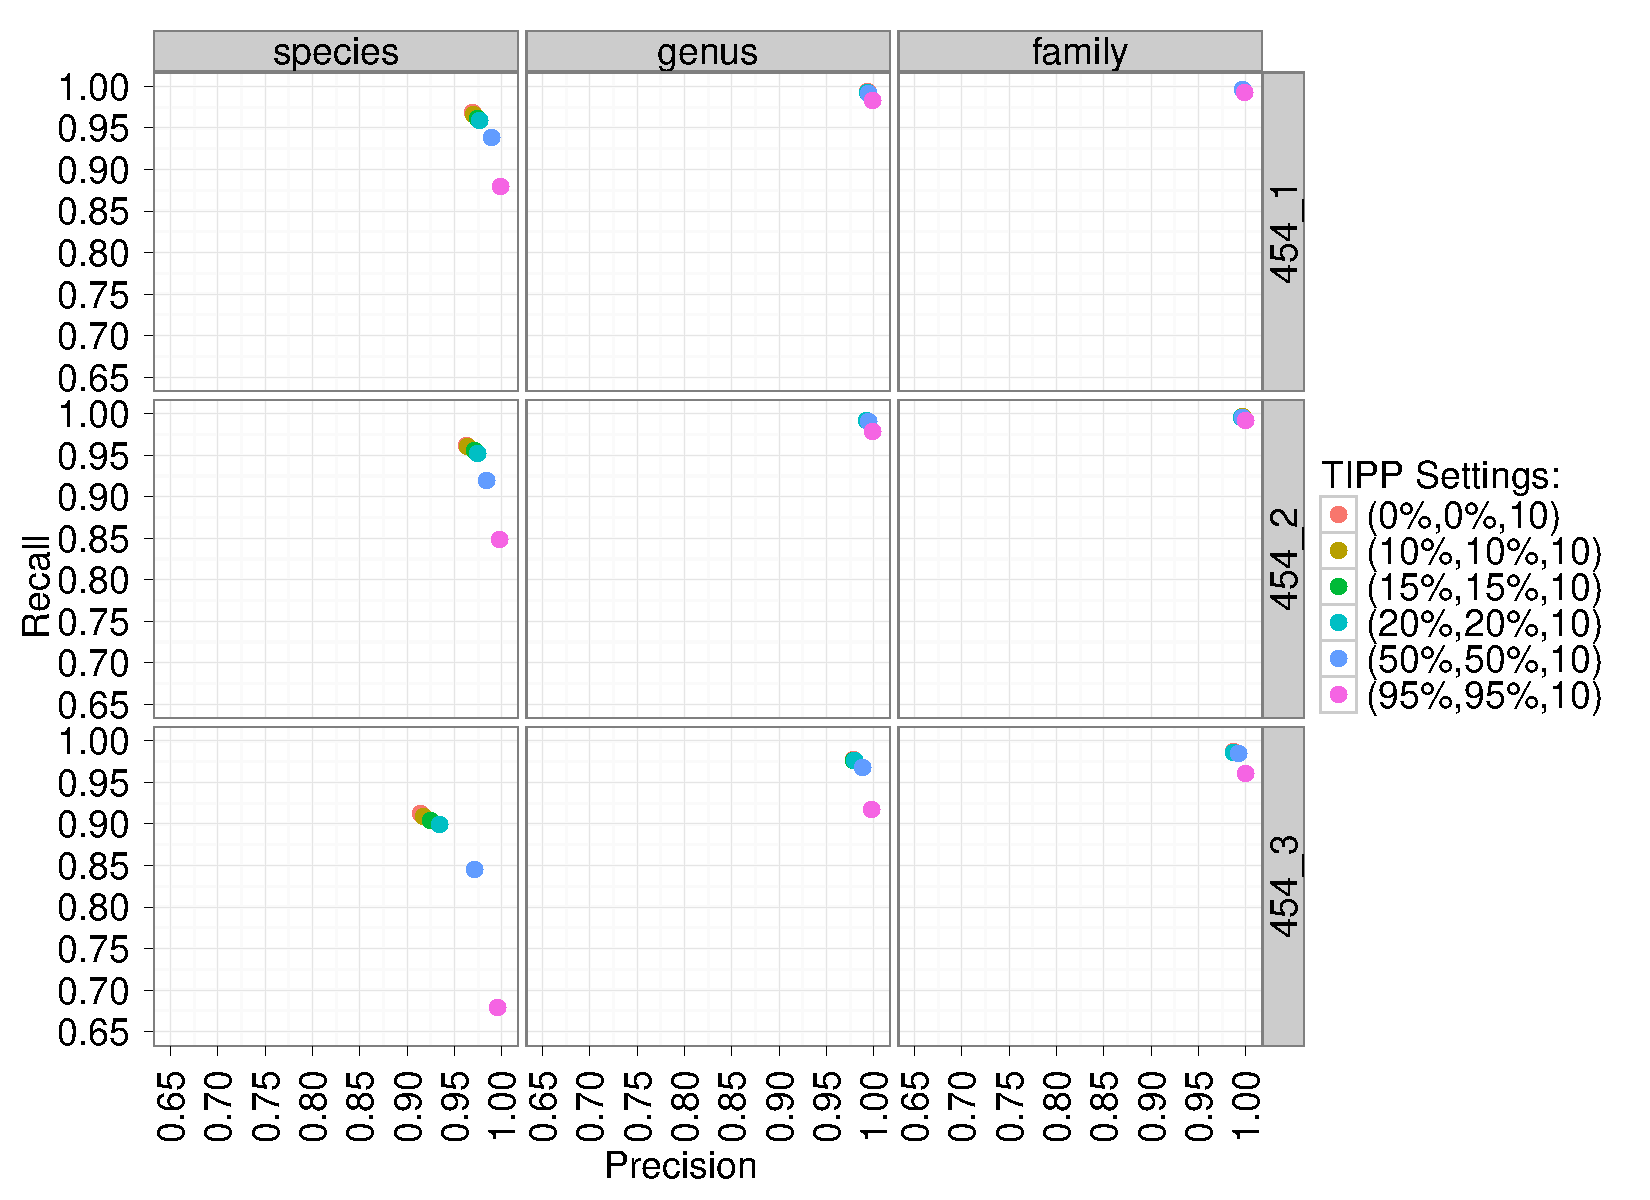
\includegraphics[scale=0.40]{higher_error/roc_higher_error_illumina_all_1_5_12}
\end{center}
%\begin{center}
%\subfigure[454-like fragments]{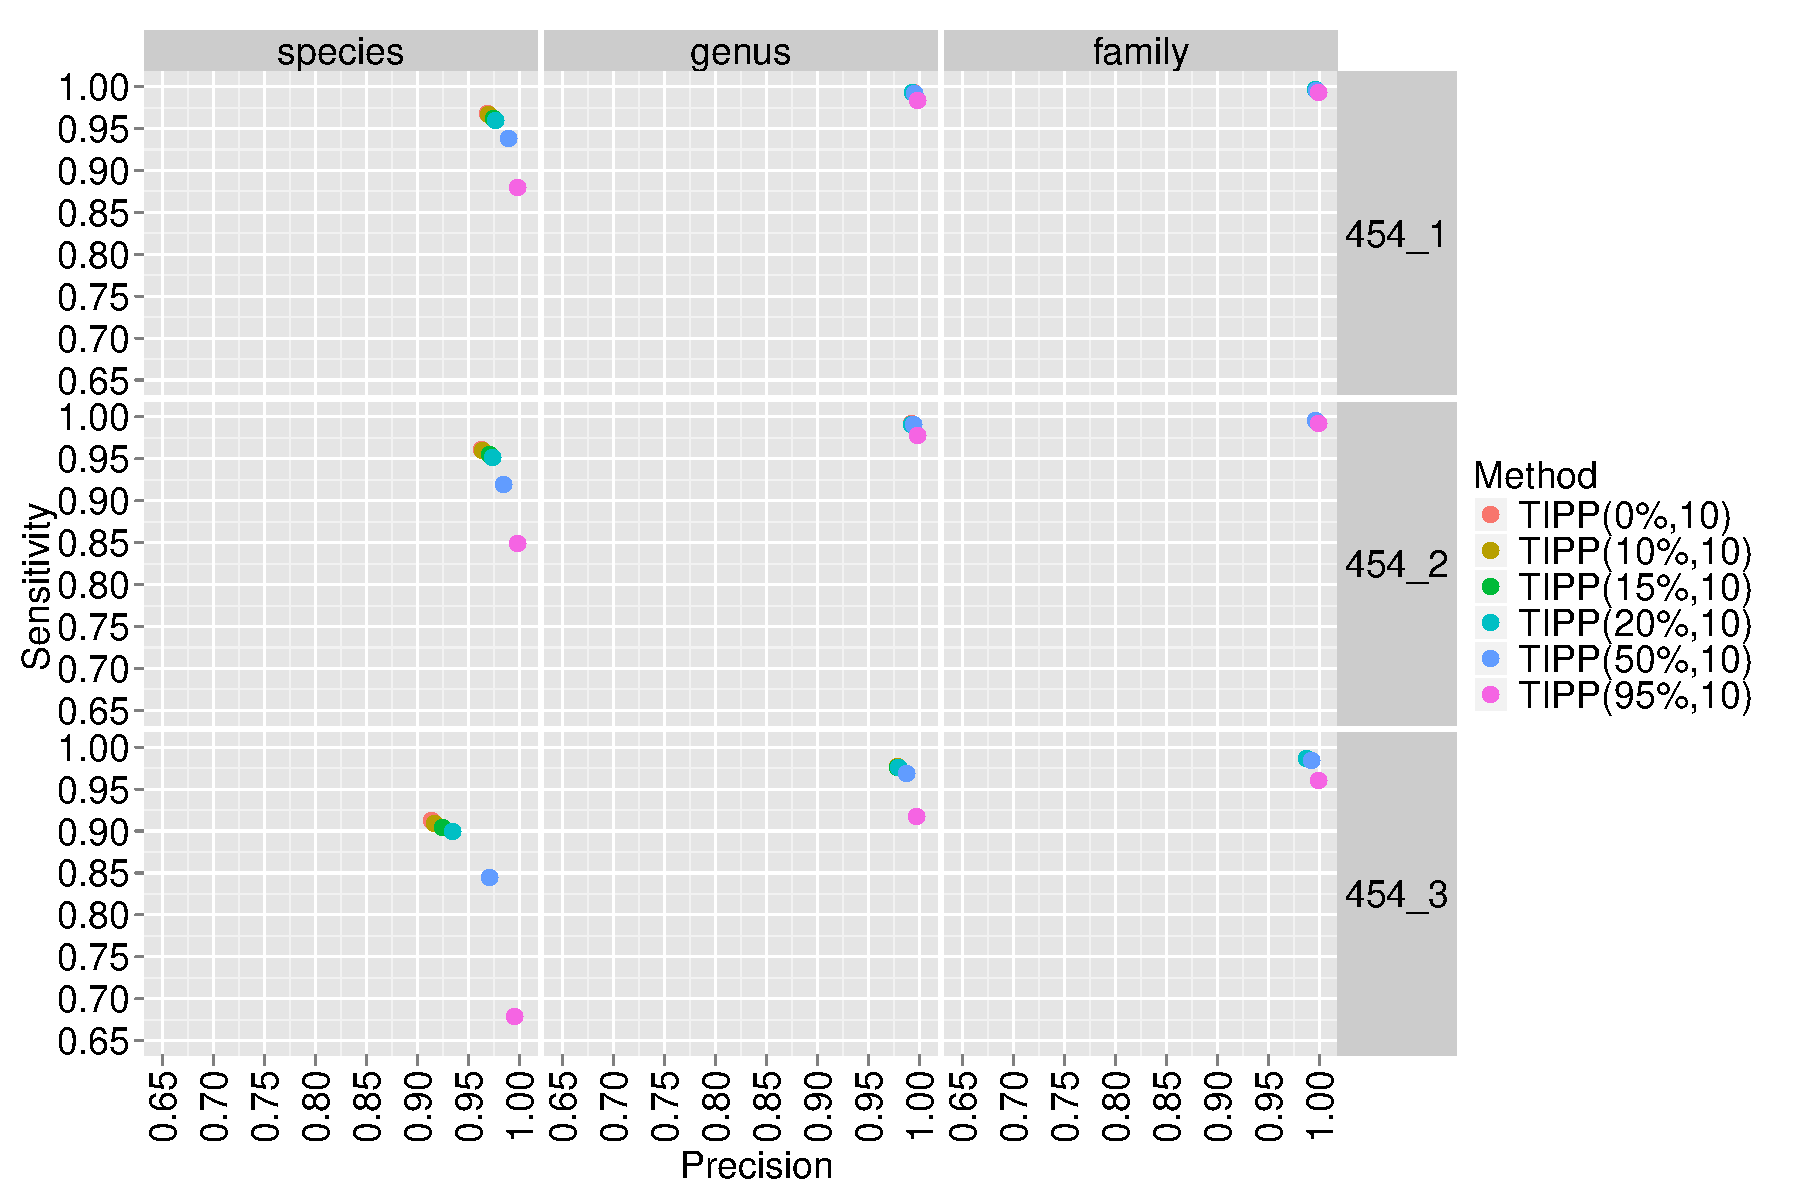
\includegraphics[scale=0.300]{higher_error/roc_higher_error_454_all_1_5_12}}\\
%\end{center}
\caption[ROC curve for TIPP on rpsB data]{\label{tipp:roc_curve_full}ROC curve showing the
  impact of the different support thresholds on precision and recall
  for species-level to family-level classification of
  fragments simulated from the rpsB marker genes in a
  non-leave-one-out experiment under the Illumina-error models. 
Note TIPP(0\%,0\%,10) is the same as 
SEPP with alignment subset size $m_a=10$.
%TIPP($X$\%,$Y$) refers to TIPP run under the
%  default settings with an alignment and placement support of $X$ and
%  an alignment decomposition subset size of $Y$.  Each column is the
%  ROC curve for a taxonomic rank and each row is the error model
%  used.
}
\end{figure}

\newpage
\subsection{Leave-one-out TIPP versus Metaphyler}  
Next, to compare TIPP and MetaPhyler, we performed a
leave-one-out study  on the 
30 marker genes used in the original MetaPhyler paper and
on the 16S gene.
%Figures \ref{tipp:leave_out_16} and \ref{tipp:leave_out_30M} 
Here we show results for the default setting for TIPP (i.e., TIPP(95\%,95\%,100)).

\subsubsection{Leave-one-out 30 marker genes}
Figures~\ref{tipp:leave_out_30M} shows the result for the leave-one-out
experiments for the 30 marker genes. 
TIPP has higher recall on these data than
MetaPhyler, and the differences are substantial and
statistically significant (p-values $\ll 10^{-5}$).
The comparison with respect to precision
% (i.e., false classifications)
is very interesting:
while TIPP generally had better precision in about two-thirds of
the cases,
 MetaPhyler had better precision one third of the time (except in one case, 
differences are statistically significant, p-value $\ll10^{-5}$; see Section \ref{supp:leave_one_out_tipp_meta_table}).
Furthermore, the relative performance depended on the
taxonomic level, so that
MetaPhyler had better precision
at the lower taxonomic levels,
and TIPP had better precision at the higher
taxonomic levels.

\subsubsection{Leave-one-out 16S RNA gene}
Figures~\ref{tipp:leave_out_16}
show the result for the leave-one-out experiments for the 16S rRNA
gene.  TIPP classifies more fragments correctly
than MetaPhyler on these data, especially at the lower taxonomic levels.
MetaPhyler generally had very low false classification
rates.  TIPP's false classification
rates were generally low, except 
when a taxonomic clade at the family or higher level is removed 
and classification is tested at the next taxonomic level.
A detailed analysis of these cases revealed that
the false classifications were mostly due
to peculiarities in the taxonomy,
potentially due to sparse taxonomic 
sampling.  

For example, in the 16S Archaea taxonomy, the Halobacteria class has exactly one family.  Therefore, the leave-one-family-out experiment results in an imbalanced taxonomy with no sequences from the Halobacteria class present in the taxonomy, and the nearest relatives are at the phylum level.  As a result, it is impossible to correctly classify the fragments at the order or class level.  Because TIPP tends to classify fragments if it can do so with some confidence, this results in a higher false classification rate (see Section~\ref{supp:archaea} for more detailed discussion).  

MetaPhyler generally had better precision than
TIPP, but at a substantial cost in recall, especially
at the lower taxonomic levels.
For example, in the leave-out-species
experiments for the 454 bacterial 16S rRNA fragments, MetaPhyler
classified only 15\% correctly at the genus level, and TIPP
classified 69\% correctly.  On the other hand, the false
classification rate for MetaPhyler was quite low, varying from
less than 1\% to 3\%, while the false classification rate for
TIPP was somewhat higher.  On the bacterial 16S rRNA gene
set, the false classification rate for TIPP was quite low
(with the exception of the phylum level in the leave-one-class-out
experiment). On the archaeal 16S rRNA genes, 
TIPP generally had low false classification rates, but
there were a few cases
where TIPP had high false classification rates.

\begin{figure}[htpb]
\begin{center}
%\mbox{
%\subfigure[Illumina error model\label{tipp:leave_out_30M_i}]{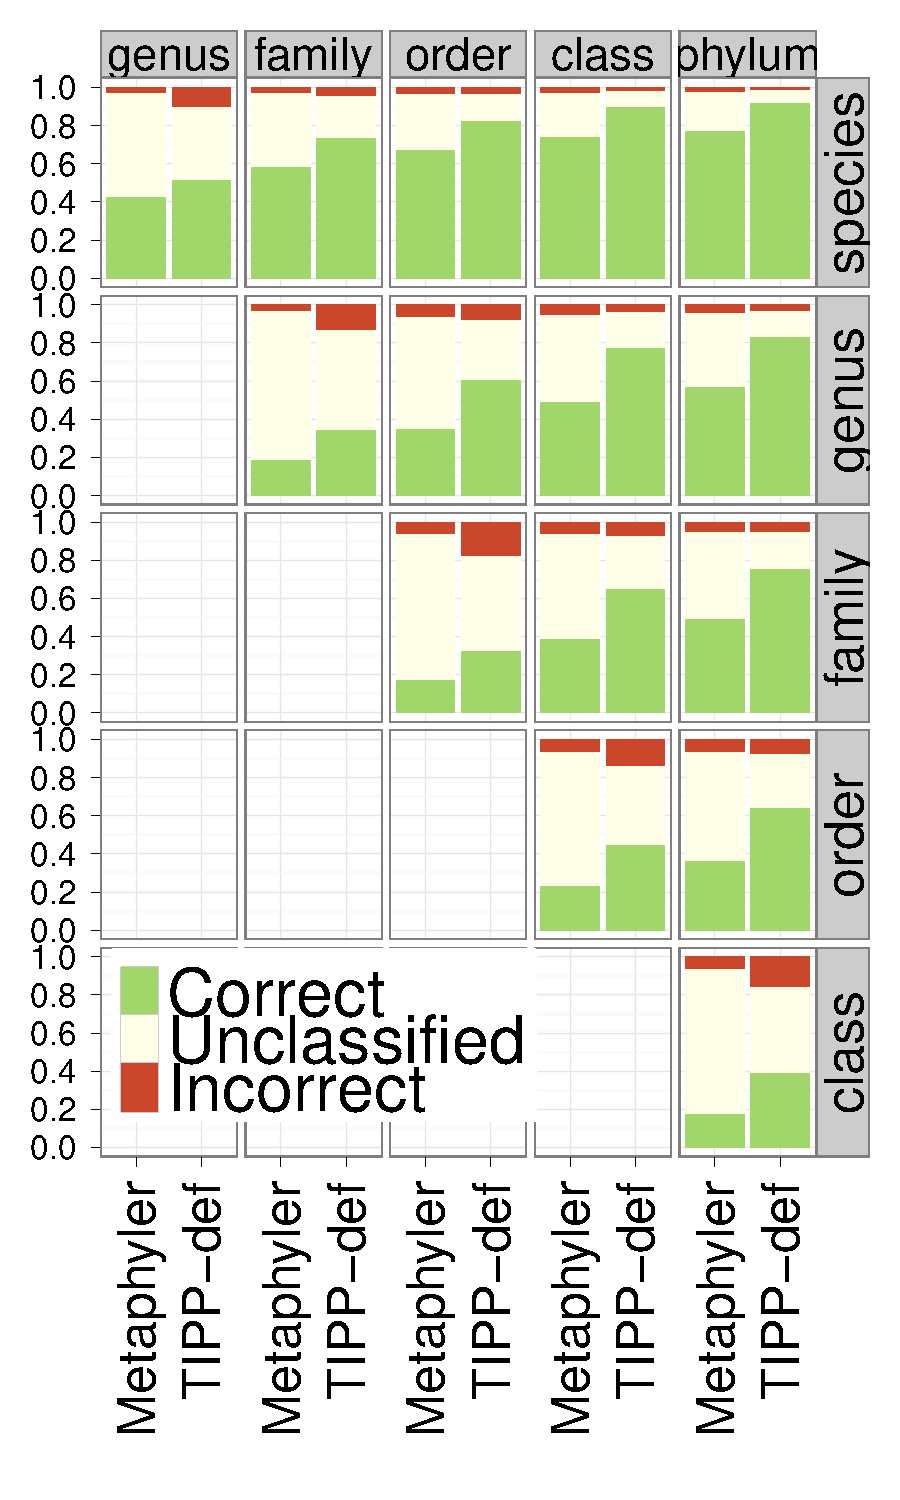
\includegraphics[scale=0.3]{{leaveout/leaveout.illumina}.pdf}}
\hspace{-14pt}
%\subfigure[454 error model\label{tipp:leave_out_30M_4}]{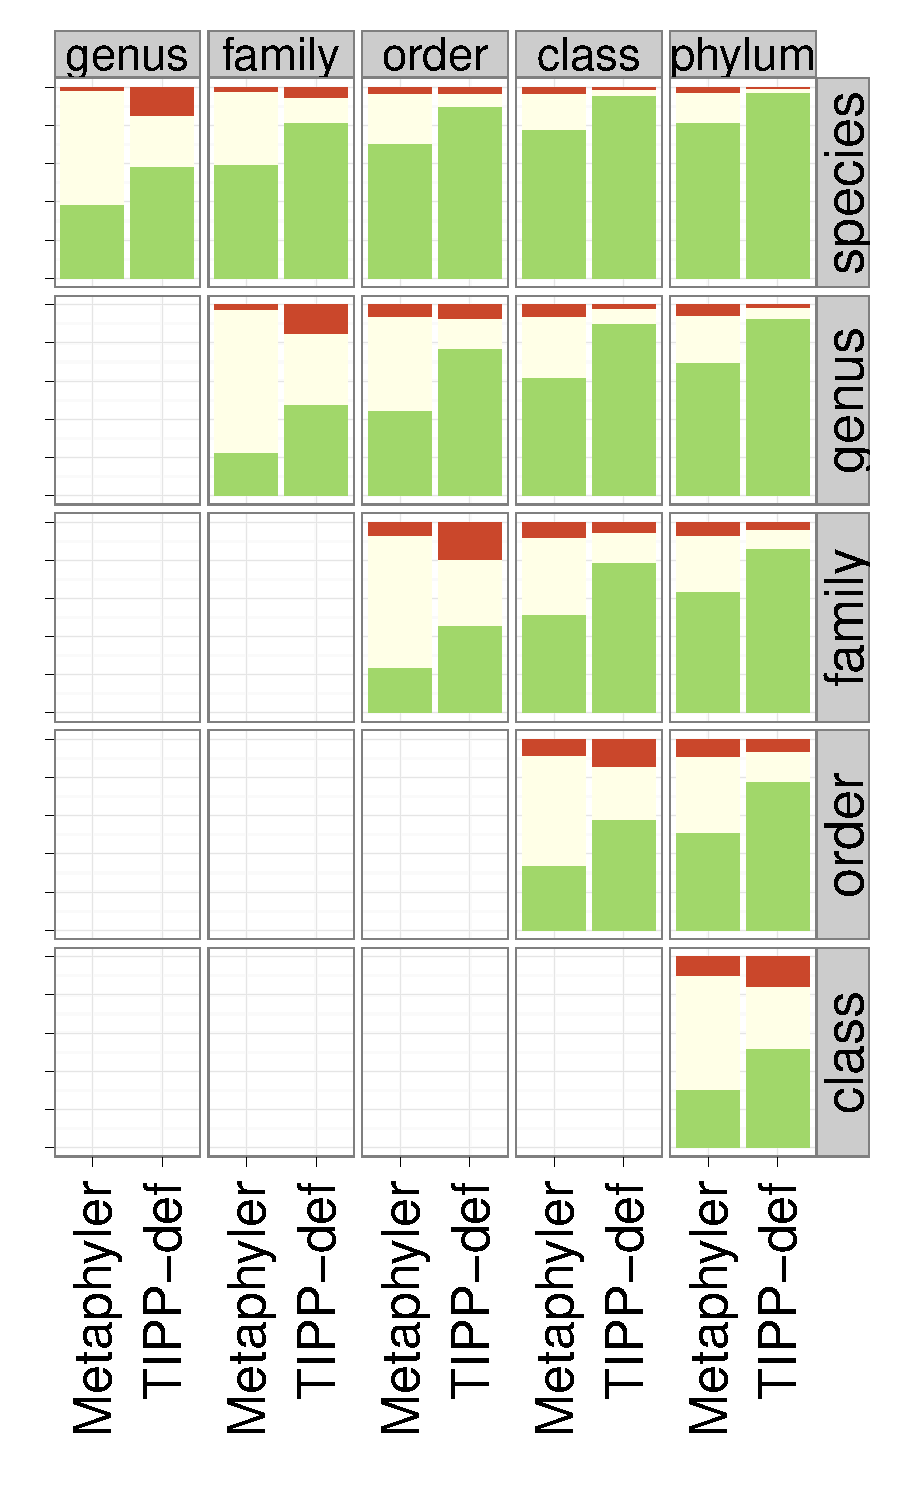
\includegraphics[scale=0.3]{{leaveout/leaveout.454}.pdf}}}
\end{center}

\caption{\label{tipp:leave_out_30M} Leave-one-out experiment
          comparing the classification accuracy for MetaPhyler
          versus TIPP-default 
(i.e.,  TIPP-default refers to TIPP(95\%,95\%,100))
on the 30 marker genes.
%with both Illumina-like and 454-error like errors.  
}
%Each column is the classification accuracy
%  for a taxonomic rank and each row the level left out.
%  TIPP($X$\%,$Y$) refers to TIPP run under the default settings with
%  an alignment support and placement support of $X$ and alignment
%  decomposition set size of $Y$.  }
\end{figure}

\begin{figure*}[htpb]
\begin{center}

%\subfigure[16S bacteria; Illumina error\label{tipp:leave_out_16_bacteria_i}]{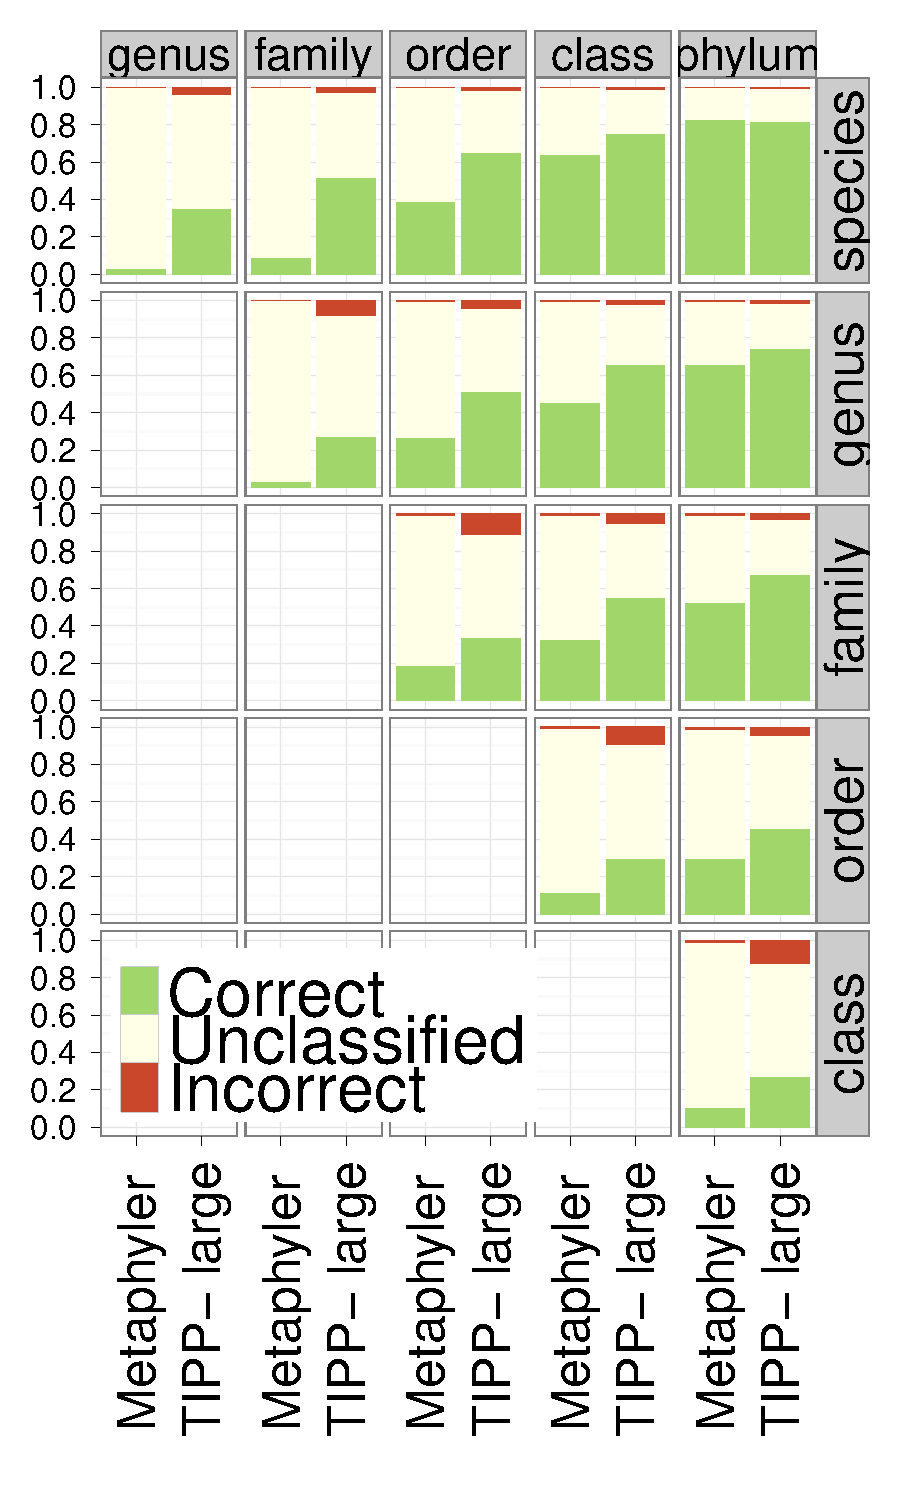
\includegraphics[scale=0.300]{{leaveout/leaveout.illumina.16S_bacteria}.pdf}}
\hspace{-14pt}
%\subfigure[16S bacteria; 454 error\label{tipp:leave_out_16_bacteria_4}]{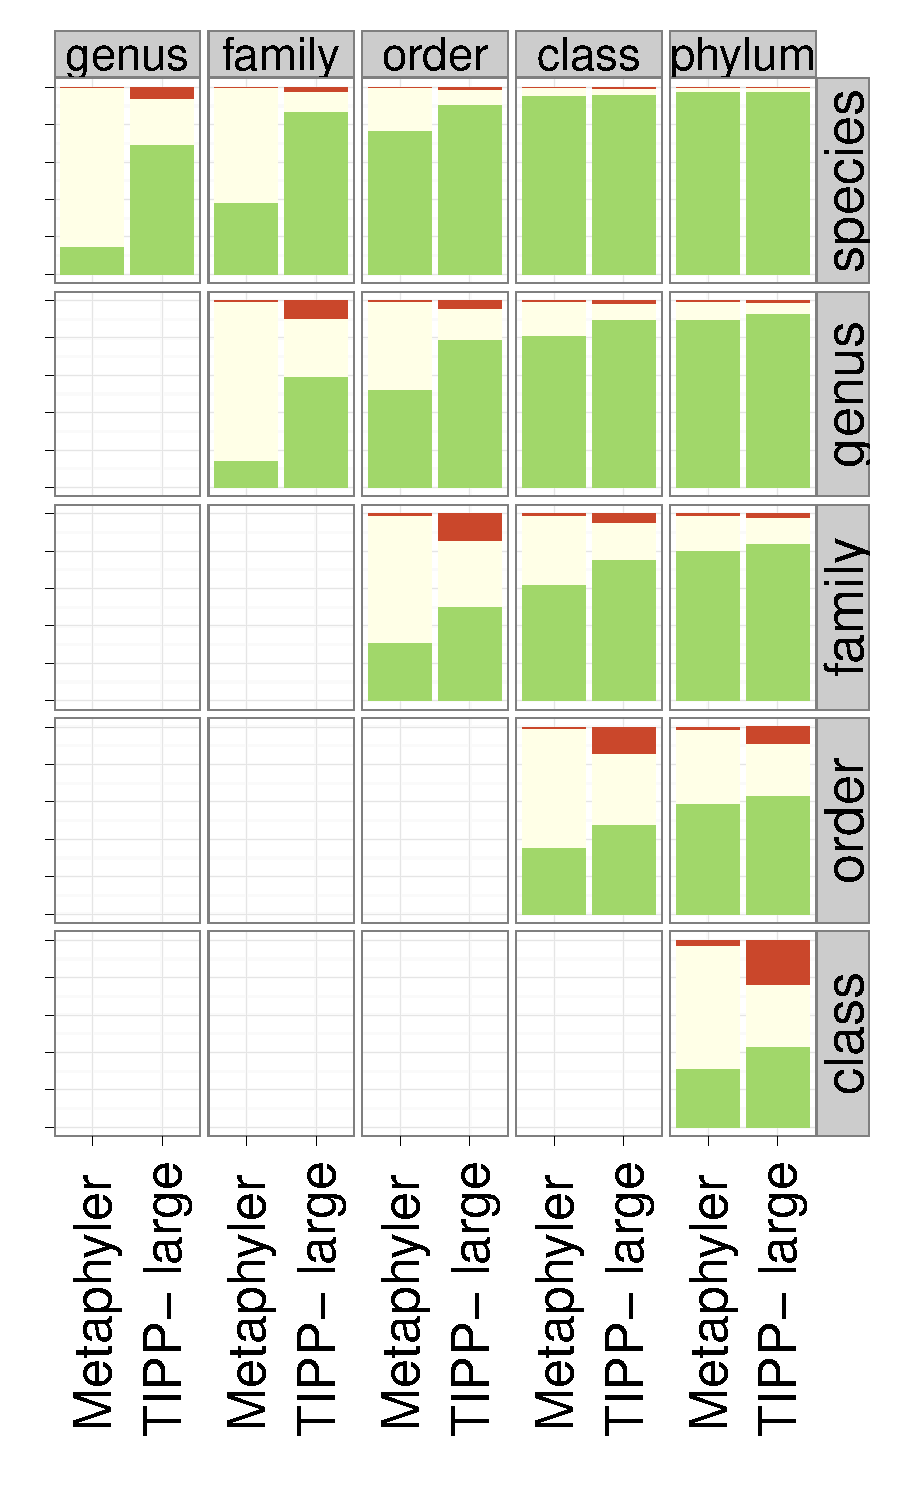
\includegraphics[scale=0.300]{{leaveout/leaveout.454.16S_bacteria}.pdf}}
%\subfigure[16S archaea; Illumina error\label{tipp:leave_out_16_archaea_i}]{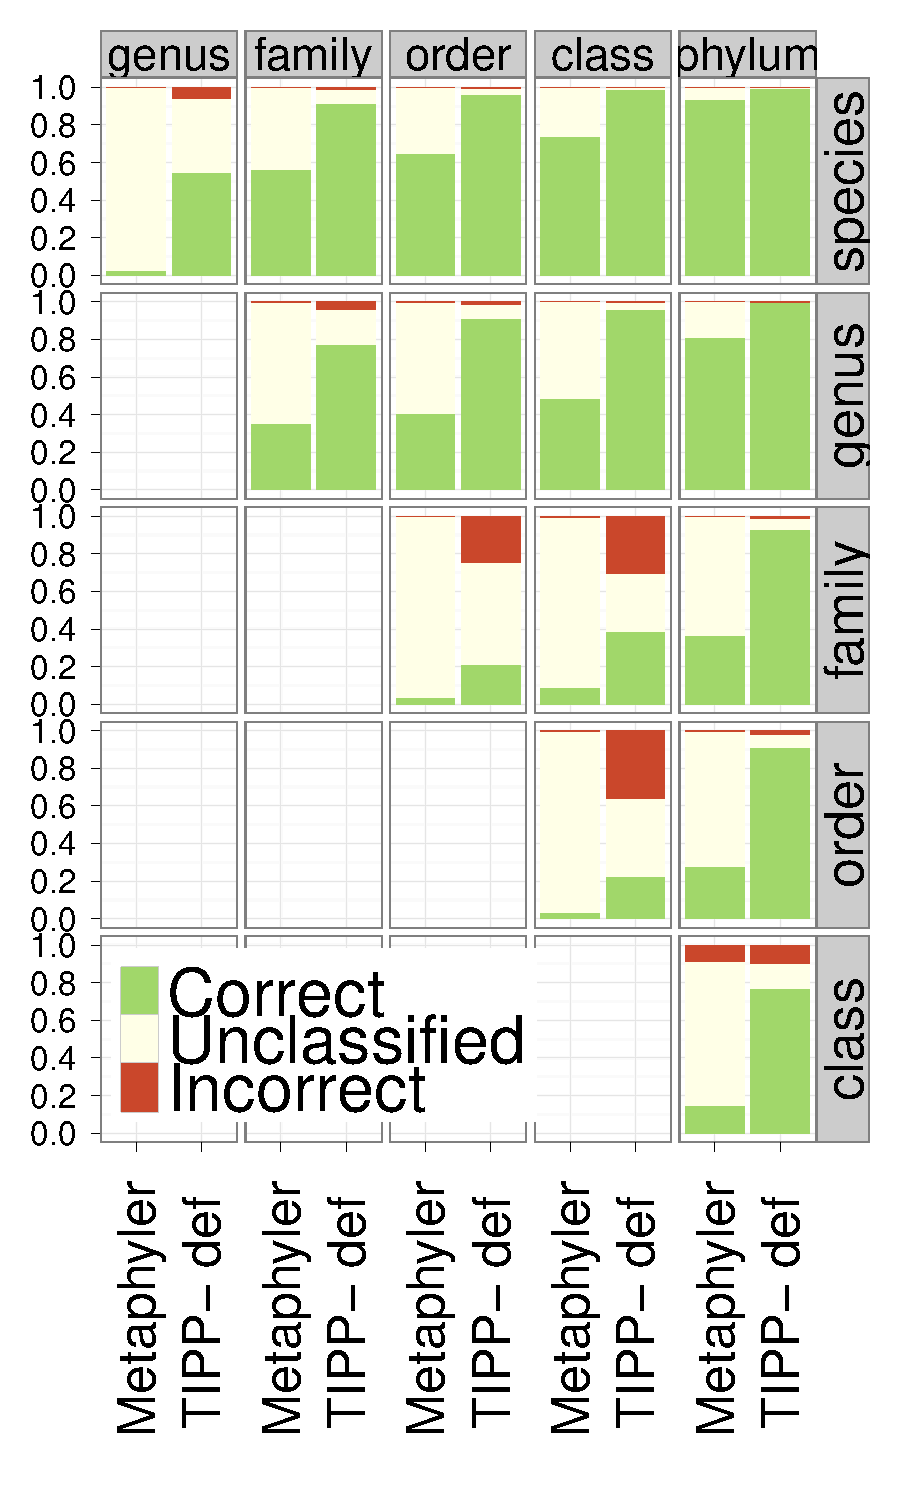
\includegraphics[scale=0.30]{{leaveout/leaveout.illumina.16S_archaea}.pdf}}
\hspace{-14pt}
%\subfigure[16S archaea; 454 error\label{tipp:leave_out_16_archaea_4}]{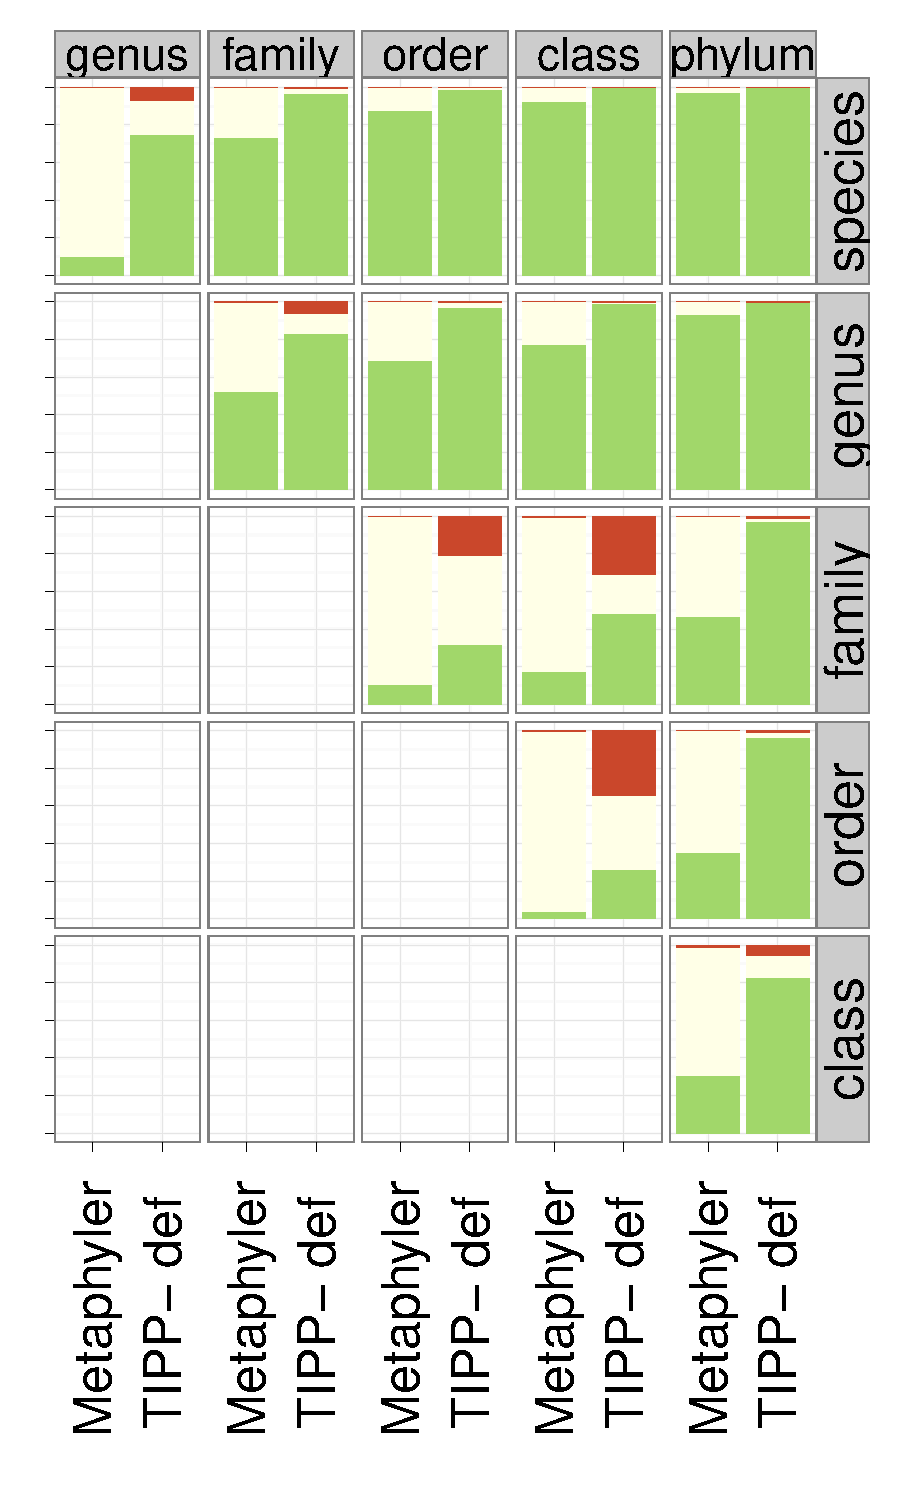
\includegraphics[scale=0.30]{{leaveout/leaveout.454.16S_archaea}.pdf}}

\end{center}
\caption{\label{tipp:leave_out_16} Leave-one-out experiment
          comparing MetaPhyler
          to TIPP on the 16S bacteria (a-b) and 16S archaea (c-d) datasets,
          with both Illumina-like and 454-like error models.
    TIPP-def refers to TIPP run
          under the default settings (i.e. TIPP(95\%,95\%,100)).
          TIPP-large is similar to TIPP-def, except placement size is set to 1,000, and the taxonomic tree is used for alignment decomposition.}
\end{figure*}

\subsection{16S RNA on archaea, leave-one-out experiments; effects of Halobacteria}\label{supp:archaea}
In this section we discuss the particularly high false 
classification rates for the leave-family-out 
and leave-order-out experiments for 16S RNA on archaea ().  
We find that the majority of the false classifications are caused by the Halobacteria class,
and  37\% of all fragments from the 16S RNA on Archaea dataset
belong to this class.  
For the leave-family-out experiment, 
the total numbers of incorrect classifications for 
TIPP(95\%,95\%,100) at the order level and class level 
were 13,651 and 18,456, respectively.  
Of those incorrect classifications, 9,223 of the 13,651 (68\%) and 
15,187 of the 18,456 (82\%) belong to fragments from this class.

Figure~\ref{tipp:taxonomy} highlights the reason for the large number of incorrect classifications.  Most normal OTUs have more than direct child OTU, i.e. phyla typically have more than one class, and classes typically have more than one order.  The Halobacteria class has only one order, and that order has only one family.  Thus, removing either the family or the order prunes the entire class from the taxonomy.  This makes it impossible to correctly classify fragments at either the order level or the class level.  Note that this phenomenon is not unique to Halobacteria:  any OTU that has exactly one direct child OTU will 
be removed completely when the child OTU is omitted in the 
leave-one-out experiment.  
This is most notable in Halobacteria because of the large number of fragments belonging to this class.

Figure~\ref{tipp:remove_class} shows the result of omitting fragments from this class from the leave-family-out and leave-order-out experiments.  When Halobacteria is omitted, the incorrect classification rate drops and is in line with the incorrect classification rates for the 16S experiments.
\begin{figure}[htpb]
\begin{center}
{\includegraphics[scale=0.35]{{leaveout/taxonomy2}.pdf}}
\end{center}
\vspace{-8pt}
\caption{\label{tipp:taxonomy} Taxonomy for Halobacteria class for the 16S RNA gene.
}
\end{figure}

\begin{figure}[htpb]
\begin{center}
%\subfigure[Illumina-like fragments]{\includegraphics[scale=0.300]{leaveout/{leaveout.illumina.no_110.16S_archaea}.pdf}}\\
\end{center}
\begin{center}
%\subfigure[454-like fragments]{\includegraphics[scale=0.300]{leaveout/{leaveout.454.no_110.16S_archaea}.pdf}}\\
\end{center}
\caption[Removing Halobacteria class from leave-family-out and leave-order-out experiments.]{\label{tipp:remove_class}Removing Halobacteria class from leave-family-out and leave-order-out experiments for 16S RNA archaea gene for fragments simulated with (a) Illumina-like errors and (b) 454-error like errors.  Each column is the classification accuracy for a taxonomic rank and each row is level being omitted.}
\end{figure}
\clearpage
\subsection{Experiment 2: Abundance profiling experiments}
We show the impact of alignment and placement support on abundance 
profiling (Fig.~~\ref{tipp:profile_short_tipp_compare} and 
\ref{tipp:profile_long_tipp_compare}).  
Although results depended on the particular dataset, 
the following trends can be observed.
On the short fragment datasets,
on average
 using the 0\% threshold improved average abundance profiles 
at the lower taxonomic levels
and was neutral at the phylum level.
On the long fragment datasets, the change in threshold had
essentially no impact.  This result lead us to select TIPP(0\%,0\%,100) for abundance profiling.


\begin{figure*}[htpb]
\begin{center}
{\includegraphics[scale=0.7]{{profiles/profiles.shortsequences.fp.tipp}.pdf}}
\end{center}
\caption{\label{tipp:profile_short_tipp_compare} Abundance profiling results comparing different TIPP methods on short fragments.  The RMSE has been normalized by TIPP(0\%,0\%,100)'s RMSE.  }
\end{figure*}


\begin{figure*}[htpb]
\begin{center}
{\includegraphics[scale=0.7]{{profiles/profiles.longsequences.fp.tipp}.pdf}}
\end{center}
\caption{\label{tipp:profile_long_tipp_compare} Abundance profiling results comparing different TIPP methods on long fragments.  The RMSE has been normalized by TIPP(0\%,0\%,100)'s RMSE.  }
\end{figure*}

In the main paper, we compare TIPP-default against other abundance profiling methods.  The tabular results for the figures are shown in Tables~\ref{tipp:table_abundance_short} and \ref{tipp:table_abundance_long}.

%Table has been updated with the new scoring metric
\begin{table}[hptb]
\caption[Normalized $RMSE$ for different methods on short fragment datasets.]{\label{tipp:table_abundance_short}
The $RMSE$ for different methods on the short fragment datasets, normalized by TIPP(0\%,0\%,100)'s $RMSE$ for each model condition and each taxonomic rank.  Thus methods with $RMSE>1$ have worse performance than TIPP, and methods with $RMSE<1$ have better performance than TIPP.  Note that PhymmBL does not output species level classification.   \textbf{fix size!}}
\begin{center}
\scalebox{0.7}{
\begin{tabular}{|l|r|r|r|r|r|r|}
\hline
Dataset&Species&Genus&Family&Order&Class&Phylum\\
{\bf FACs HC Illumina}&&&&&&\\
\hline
NBC&1.889&2.278&2.226&2.241&1.431&3.111\\
PhymmBL&NA&2.254&2.186&2.201&1.405&3.035\\
MetaPhlAn&1.134&1.101&1.403&1.054&0.967&2.018\\
MetaPhyler&5.324&2.095&1.496&1.351&1.279&0.743\\
TIPP(0\%,0\%,100)&1.000&1.000&1.000&1.000&1.000&1.000\\
TIPP(95\%,95\%,100)&1.341&1.264&1.101&1.104&1.119&0.691\\
\hline
{\bf WebCarm Illumina}&&&&&&\\
\hline
NBC&1.132&1.483&2.768&2.806&4.116&8.142\\
PhymmBL&NA&1.492&2.693&2.589&3.508&6.052\\
MetaPhlAn&1.321&1.576&1.377&2.229&2.720&5.595\\
MetaPhyler&3.443&1.816&2.181&1.738&1.759&1.630\\
TIPP(0\%,0\%,100)&1.000&1.000&1.000&1.000&1.000&1.000\\
TIPP(95\%,95\%,100)&1.066&0.899&0.999&1.141&1.065&1.773\\
\hline
{\bf MetaPhlAn HC}&&&&&&\\
\hline
NBC&1.200&2.066&2.192&2.474&2.234&1.985\\
PhymmBL&NA&2.061&2.210&2.500&2.217&2.023\\
MetaPhlAn&0.585&0.742&0.833&0.822&0.769&0.445\\
MetaPhyler&5.037&2.165&1.307&1.268&1.186&1.103\\
TIPP(0\%,0\%,100)&1.000&1.000&1.000&1.000&1.000&1.000\\
TIPP(95\%,95\%,100)&1.176&1.028&1.035&1.060&1.093&1.094\\
\hline
{\bf MetaPhlAn LC}&&&&&&\\
\hline
NBC&2.020&2.175&2.644&2.483&2.205&1.708\\
PhymmBL&NA&2.200&2.624&2.462&2.132&1.675\\
MetaPhlAn&0.492&0.527&0.725&0.952&0.787&0.628\\
MetaPhyler&10.000&7.744&4.169&2.051&1.880&1.803\\
TIPP(0\%,0\%,100)&1.000&1.000&1.000&1.000&1.000&1.000\\
TIPP(95\%,95\%,100)&1.286&0.919&0.789&0.967&1.044&1.004\\
\hline
{\bf Average}&&&&&&\\
\hline
NBC&1.595&1.991&2.435&2.440&2.038&2.661\\
PhymmBL&NA&1.993&2.403&2.386&1.934&2.487\\
MetaPhlAn&0.931&1.029&1.128&1.184&1.103&1.333\\
MetaPhyler&6.143&3.642&2.310&1.604&1.460&1.278\\
TIPP(0\%,0\%,100)&1.000&1.000&1.000&1.000&1.000&1.000\\
TIPP(95\%,95\%,100)&1.211&1.030&0.988&1.064&1.092&0.997\\
\hline
\end{tabular}}
\end{center}
\end{table}


\begin{table}[hptb]
\caption[Normalized $RMSE$ for different methods on long fragment datasets.]{\label{tipp:table_abundance_long}
The $RMSE$ for different methods on the long fragment datasets, normalized by TIPP(0\%,0\%,100)'s $RMSE$ for each model condition and each taxonomic rank.  Thus methods with $RMSE>1$ have worse performance than TIPP, and methods with $RMSE<1$ have better performance than TIPP.  Note that PhymmBL does not output species level classification.   \textbf{fix size!}}
\begin{center}
\scalebox{0.7}{
\begin{tabular}{|l|r|r|r|r|r|r|}
\hline
Dataset&Species&Genus&Family&Order&Class&Phylum\\
{\bf FACs HC}&&&&&&\\
\hline
NBC&1.554&1.864&2.008&2.030&1.397&3.124\\
PhymmBL&NA&1.727&1.869&1.885&1.236&2.593\\
MetaPhlAn&1.220&1.087&1.533&1.239&0.661&1.720\\
MetaPhyler&5.338&2.048&1.441&1.366&1.176&1.268\\
TIPP(0\%,0\%,100)&1.000&1.000&1.000&1.000&1.000&1.000\\
TIPP(95\%,95\%,100)&1.007&1.002&0.967&0.977&1.028&1.134\\
\hline
{\bf FAMeS HC}&&&&&&\\
\hline
NBC&0.797&0.894&0.830&0.784&0.661&1.630\\
PhymmBL&NA&0.870&0.783&0.732&0.584&1.399\\
MetaPhlAn&1.206&0.834&0.761&0.608&0.478&0.877\\
MetaPhyler&4.159&1.624&1.194&1.109&1.249&1.777\\
TIPP(0\%,0\%,100)&1.000&1.000&1.000&1.000&1.000&1.000\\
TIPP(95\%,95\%,100)&1.025&1.002&1.005&0.998&0.988&0.983\\
\hline
{\bf FAMeS LC}&&&&&&\\
\hline
NBC&0.974&0.943&1.006&0.976&0.658&1.127\\
PhymmBL&NA&1.016&0.527&0.528&0.334&0.713\\
MetaPhlAn&3.849&2.714&1.813&1.868&1.349&1.683\\
MetaPhyler&6.489&2.197&1.442&1.221&1.175&1.331\\
TIPP(0\%,0\%,100)&1.000&1.000&1.000&1.000&1.000&1.000\\
TIPP(95\%,95\%,100)&1.195&1.046&1.036&1.008&1.015&0.997\\
\hline
{\bf FAMeS MC}&&&&&&\\
\hline
NBC&1.844&1.829&1.651&1.679&1.363&1.863\\
PhymmBL&NA&1.645&1.342&1.363&1.069&1.461\\
MetaPhlAn&2.332&1.521&0.690&0.859&0.647&2.463\\
MetaPhyler&4.997&1.741&1.291&1.260&1.019&2.366\\
TIPP(0\%,0\%,100)&1.000&1.000&1.000&1.000&1.000&1.000\\
TIPP(95\%,95\%,100)&1.014&1.015&1.049&1.037&1.038&0.987\\
\hline
{\bf WebCarma}&&&&&&\\
\hline
NBC&0.771&0.795&0.862&0.818&1.141&2.081\\
PhymmBL&NA&0.788&0.807&0.769&0.839&1.013\\
MetaPhlAn&1.384&1.153&1.127&1.207&1.665&1.003\\
MetaPhyler&3.205&1.467&1.318&1.186&1.567&1.260\\
TIPP(0\%,0\%,100)&1.000&1.000&1.000&1.000&1.000&1.000\\
TIPP(95\%,95\%,100)&0.932&0.894&1.039&1.038&1.071&0.957\\
\hline
{\bf Average}&&&&&&\\
\hline
NBC&1.161&1.250&1.264&1.236&1.059&1.888\\
PhymmBL&NA&1.194&1.075&1.045&0.823&1.373\\
MetaPhlAn&1.802&1.372&1.202&1.168&0.986&1.463\\
MetaPhyler&4.582&1.779&1.343&1.228&1.239&1.520\\
TIPP(0\%,0\%,100)&1.000&1.000&1.000&1.000&1.000&1.000\\
TIPP(95\%,95\%,100)&1.010&0.973&1.020&1.013&1.029&1.012\\
\hline
\end{tabular}}
\end{center}
\end{table}

\subsection{Experiment 3: Exploring robustness to sequencing error on  taxonomic identification  experiments.}

In the main paper we showed non-leave-one-out results comparing TIPP(95\%,95\%,100), MetaPhyler, PhmmBL, and NBC on all marker genes under the 454\_3 error model condition. 
Here we also show results on all remaining error model conditions. 
Figures~~\ref{tipp:comparison_methods_30M_i} and \ref{tipp:comparison_methods_30M_4} show results
 under different rates of Illumina-like and 454-like errors.
 
Figure \ref{tipp:comparison_methods_dark_matter} show results for false positive detection of ``dark matter'' under the assumption that any read left unclassified at the phylum level comes from a novel phylum.  

\begin{figure*}[htpb]
\begin{center}
%\subfigure[Illumina error model\label{tipp:comparison_methods_30M_i}]{\includegraphics[scale=0.40]{{higher_error/higher_error_illumina_comparison_4_2_14}.pdf}}
%\subfigure[Illumina error model\label{tipp:comparison_methods_30M_4}]{\includegraphics[scale=0.40]{{higher_error/higher_error_454_comparison_4_2_14}.pdf}}
\end{center}
\caption{\label{tipp:comparison_methods_all} Non-leave-one-out experiments
          comparing the classification accuracy for NBC, PhymmBL, MetaPhyler
          and TIPP-default 
(i.e.,  TIPP-default refers to TIPP(95\%,95\%,100))
for fragments simulated from the 30 marker genes under different rates of Illumina-like and 454-like errors.  Note that PhymmBL does not classify below the genus level and thus has 100\% unclassified rate at the species level.}
\end{figure*}

\begin{figure*}[htpb]
\begin{center}
\label{tipp:comparison_methods_dark}{\includegraphics[scale=0.85]{{higher_error/higher_error_comparison_dark_matter_4_2_14}.pdf}}
\end{center}
\caption{\label{tipp:comparison_methods_dark_matter} Non-leave-one-out experiments
          comparing the proportion of classified and unclassified reads at the phylum level for NBC, PhymmBL, MetaPhyler
          and TIPP-default 
(i.e.,  TIPP-default refers to TIPP(95\%,95\%,100))
for fragments simulated from the 30 marker genes under different error models.  If reads that could not be classified at the phylum level are considered novel, the unclassified rate identical to the false positive rate for detecting ``dark matter'' microbes.}
\end{figure*}

\newpage
\section{Non-leave-one-out Running Time Study.}  
In this section we report on running time experiments performed on the rpsB marker gene
in order to examine the impact of the maximum alignment decomposition size on the running time.  While the previous leave-one-out and non-leave-one out experiments had over million fragments, each individual TIPP run typically examined fewer than 5,000 fragments.  Thus, computing the total running times across all the experiments would incur a substantial cost in setup time.

To obtain a better estimate of the running time, we ran TIPP on a very large simulated dataset.  We simulated 200,000 fragments from rpsB with Illumina-like errors.  
We selected the rpsB gene because the number of
sequences in its reference alignment
is on the high end of the
range (1463), so that its running time  will
be also at the high end of most
analyses.   We ran TIPP(95\%,95\%,$X$) on the fragments, with $X$ ranging from 10 to the total number of sequences in rpsB, and
we used pplacer within TIPP to place the fragments.  
Note that we could not run EPA inside of TIPP for these experiments,
as we  found EPA to be significantly slower than pplacer.  
For example, 
the time to place 200 fragments using pplacer within TIPP was roughly 
half a minute,  while EPA took 55 minutes.

Each TIPP run was computed on an individual computer node with 32 GB of memory and was given 4 CPUs.  We report the elapsed wall clock time in Table~\ref{tipp:running_time}.  

\begin{table}[h]
\caption[Running time experiment.]{\label{tipp:running_time}Wall clock running time (in hours) to classify 
200,000 fragments for different maximum alignment decomposition sizes, using
four processors.
The fragments were simulated using MetaSim with Illumina\_1 errors from the rpsB marker gene.}
\begin{center}
\begin{tabular}{|l|r|}
\hline
Method &  Wall clock time (hr)\\
\hline
TIPP(95\%,10) & 7.5\\
TIPP(95\%,100) & 3.6\\
TIPP(95\%,500) & 2.8\\
TIPP(95\%,ALL) & 2.1\\
\hline
\end{tabular}
\end{center}

\end{table}

\newpage
\section{Alignment Support Calculation}\label{tipp:bitscores}
In the main paper, we have described how for each fragment, we align it to multiple
alignment subsets, and then take as many alignment as necessary so that 
together they provide a total support above a certain threshold.
To do this rigorously, we use HMMER output to calculate the probability
that a given fragment is generated by one of the models from 
a set of models, each associated with an alignment subset.
These calculations are all based on the assumptions that 1) alignment subsets are
disjoint, so that at most one subset generates the fragment, and 2)
the fragment does indeed belong to the gene, so that it is generated by some
alignment subset. 

\paragraph{Minimum Alignment Support Threshold. }
We now show how 
TIPP computes the probability that a fragment is
generated by a set of alignment subsets.
For a given HMMER model $H$ and fragment $x$, HMMER calculates a bit-score, defined as:
\begin{equation}
BS(H) = log_2 \frac{P(x|H)}{P(x|R)} \label{tipp:bitscore_equation}
\end{equation}
\noindent where $BS(H)$ is the bit-score for x on H, $P(x|H)$ 
is the probability of model H generating fragment $x$, and $P(x|R)$ is the probability of a random model R generating fragment $x$.
Thus models producing higher bit-scores are more likely to have generated the fragment. 


Assuming that a fragment $x$ is generated by 
exactly one  of the  HMMs $H_1$ to $H_n$ (each corresponding to a different alignment subset),
the probability that $H_i$ generated $x$ is:

\begin{equation}
P(H_i|x) = \frac{P(x|H_i)P(H_i)}{\sum_{j=1}^{n} P(x|H_j)P(H_j)}.\label{tipp:bitscore_equation_1}
\end{equation}

Assuming that uniform prior probability 
(i.e. $P(H_i)=P(H_j)$),
we can rewrite Equation~\ref{tipp:bitscore_equation_1} as:

\begin{equation}
P(H_i|x) = \frac{1}{\sum_{j=1}^{n} \frac{P(x|H_j)}{P(x|H_i)}}.\label{tipp:bitscore_equation_2}
\end{equation}

By Equation~\ref{tipp:bitscore_equation}, %$BS(H_j)-S(H_i)$ is:
 \begin{align}
{BS(H_j) - BS(H_i)}&= {\log_2 \frac{P(x|H_j)}{P(x|R)} - \log_2 \frac{P(x|H_i)}{P(x|R)}} \\=  \log_2\frac{P(x|H_j)}{P(x|H_i)}\label{tipp:bitscore_equation_4}
\end{align}

Substituting into Equation~\ref{tipp:bitscore_equation_2}, 
the result is the formula for computing the probability of $H_i$ using bit-scores:

\begin{equation}
P(H_i|x) = \frac{1}{\sum_{j=1}^{n} 2^{BS(H_j)-BS(H_i)}}
\end{equation}\label{tipp:bitscore_equation_5}
\noindent
Thus, 
assuming that the bit-scores are sorted such 
that $BS(A_i) \geq BS(A_{i+1})$ ($i=1,2,\ldots,n-1$), 
to reach a specified threshold $s_a$ we find the
smallest $m$ such that ${\sum_{k=1}^{m} P(H_k|x)} \geq s_a$.


\newpage

\section{Abundance profile calculation}\label{supp:profile_estimation}
In the main paper, we briefly described how to compute an abundance profile of a method.  We now provide more details on this procedure.  Almost all the studied methods (lone exception of NBC) can leave a fragment partially classified.  Abundance profiles at a specific level for a given method is computed by removing all unclassified fragments at the specific level and then computing the abundance profile on the remaining fragments.  For example, if the abundance profile of a method at the species level is 30\% species A, 30\% species B, and 60\% unclassified, the modified abundance profile would be 50\% species A and 50\% species B.  Note that for the marker-based methods, the source gene of the fragment is ignored when computing abundance profiles, i.e., the profiles are computing on the entire set of classified fragments, ignoring that the fragments may be binned to different markers.

\section{Dataset}

\subsection{Marker Genes and Empirical Statistics\label{tipp:marker_genes}}
Table \ref{tipp:marker_stats} shows statistics for the marker genes used in this study. 
We show the maximum and average p-distances for each gene, which are defined as
follows.  We compute the SAT\'{e} alignment on each gene, and we define the
p-distance between two aligned sequences for a gene to be the fraction of
the positions in which they both have nucleotides, but the nucleotides are different.
The maximum of these pairwise distances is the ``max p-distance", and the
average of these pairwise distances is ``average p-distance". Datasets
that have maximum p-distances at 0.75 or larger are said to be ``saturated",
and estimating alignments and trees on such datasets is very difficult.

\begin{table}[p]
\caption[Marker Gene statistics.]{\label{tipp:marker_stats}Statistics for 
30 marker genes and 16S RNA gene.  }
\begin{center}
\begin{tabular}{|l|r|r|r|}
\hline
Marker & Number of sequences & Max p-distance & Average p-distance \\
\hline
16S\_archaea & 375 & 0.35 & 0.22 \\
16S\_bacteria & 9197 & 0.36 & 0.20 \\
dnaG & 1555 & 1.00 & 0.59 \\
frr & 1313 & 0.67 & 0.47 \\
infC & 1338 & 0.73 & 0.46 \\
nusA & 1406 & 1.00 & 0.56 \\
pgk & 1544 & 0.81 & 0.49 \\
pyrG & 1501 & 1.00 & 0.43 \\
pyrg & 65 & 0.55 & 0.43 \\
rplA & 1396 & 0.70 & 0.45 \\
rplB & 1370 & 0.68 & 0.43 \\
rplC & 1400 & 0.73 & 0.48 \\
rplD & 1341 & 0.75 & 0.53 \\
rplE & 1399 & 0.72 & 0.42 \\
rplF & 1366 & 0.78 & 0.48 \\
rplK & 1421 & 1.00 & 0.41 \\
rplL & 1315 & 0.77 & 0.42 \\
rplM & 1365 & 0.71 & 0.45 \\
rplN & 1311 & 0.66 & 0.40 \\
rplP & 1351 & 0.75 & 0.43 \\
rplS & 1383 & 0.81 & 0.46 \\
rplT & 1279 & 0.73 & 0.44 \\
rpmA & 1223 & 0.63 & 0.42 \\
rpsB & 1463 & 0.74 & 0.45 \\
rpsC & 1293 & 1.00 & 0.46 \\
rpsE & 1316 & 0.69 & 0.45 \\
rpsI & 1174 & 0.74 & 0.47 \\
rpsJ & 1287 & 0.68 & 0.41 \\
rpsK & 1308 & 0.64 & 0.42 \\
rpsM & 1307 & 0.70 & 0.43 \\
rpsS & 1277 & 0.67 & 0.40 \\
smpB & 1278 & 0.71 & 0.49 \\
\hline
\end{tabular}
\end{center}

\end{table}


\subsection{Fragments}
We used MetaSim \cite{Richter2008} to 
generate fragments, starting from the reference
datasets of
 30 marker genes and the 16S gene.
Both 100-bp Illumina-type fragments and 
300-bp 454-type fragments were generated,
with different levels of error (thus, we have Illumina\_1, Illumina\_2,
and
Illumina\_4 models for Illumina-type error, and similarly
454\_1, 454\_2, and 454\_3 models).  The index $j$ in Illumina\_$j$ error model is scaling factor
for the substitution error rates; an index of 2 means all the substitution error rates per site
are doubled.  The index $j$ in the 454\_$j$ error model is the scaling factor for the negative flow error rate; an index of 2 means that insertions are twice more likely.
Illumina-type fragments contained only substitution errors,
and  454-type fragments contained only indel errors, biased toward insertions.
The Illumina\_1  and 454\_1 models
have the lowest error rates, and the
Illumina\_4 and 454\_3 models have
the highest error rates.  
Table \ref{tipp:metasim_stats} shows the amount of error simulated for each model condition. 

\begin{table}[h]
\caption[Higher error fragment statistics.]{\label{tipp:metasim_stats}Statistics for non-leave-one-out fragment datasets.  
Fragments were simulated using MetaSim with Illumina-like error or 
with 454-like errors.  %For each dataset, 100,000 fragments were simulated.  
Illumina-like fragments suffered from single bp substitution errors, while 454-like fragments suffered from indel errors, biased toward insertions. }  %Thus, increasing the error rates for the Illumina-simulated fragments did not change the fragment length, but increasing the error rates for the 454-simulated fragments resulted in longer fragments.}
\begin{center}
\begin{tabular}{|l|r|r||l|r|r|}
\hline
Model &  Num. substitutions &  Avg.  & Model  & Num. indel events &  Avg.  \\
name&   per fragment (avg) &       length&         name &  per fragment (avg) &  length \\
\hline
Illumina\_1 & 0.5                          & 100                   & 454\_1      & 14.2                        & 272.5                    \\ 
Illumina\_2 & 1.5                          & 100                    &454\_2      & 24.5                        & 275.9                    \\ 
Illumina\_4 & 3.8                          & 100                    &454\_3      & 60.2                        & 284.9                    \\ 
\hline
\end{tabular}
\end{center}
\end{table}
\newpage
\section{Abundance Profile Datasets\label{tipp:datasets}}
\subsection{Metaphlan Simulated Dataset}  
The Metaphlan simulated datasets~\cite{Segata2012a} consist of 2 high complexity datasets and 8 low complexity datasets.  The high complexity datasets contain 1,000,000 fragments each, and the low complexity datasets contain 250,000 fragments each.  The average read length of the datasets was 88 bps.  The fragments span the bacteria and archaea domains.

\subsection{FACs HC}  
The FACs simulated dataset~\cite{Stranneheim2010} is a high complexity dataset containing 19 bacterial genomes, 3 viral genomes, and 2 human chromosomes.  All genomes are present in equal amounts.  MetaSim was used to simulate 454-like fragments from the genomes.  The dataset contained 100,000 sequences total with an average length of 269 bps. The fragments in the original dataset span the bacterial, viral, and eukaryote domains.  We used only the bacterial fragments from this dataset.

We also generated a high complexity dataset with 300,000 Illumina-like reads using MetaSim from this dataset.  The fragments had an average length of 100 bps.

\subsection{FAMeS}  
The FAMeS simulated datasets~\cite{Mavromatis2007} consist of a low complexity, medium complexity, and high complexity dataset.  Fragments were obtain from isolate genome sequencing projects at the Department of Energy Joint Genome Institute (DOE-JGI).  Simulated abundance profiles were created by adding the desired proportion of fragments to achieve a desired profile.  Thus, while the sequences are from a real study, the abundance profile itself is simulated and the true abundance is known.  The datasets consist of 328,728 sequences total with an average length of 950 bps.  The fragments span the bacterial and archaeal domains of life. 

\subsection{WebCarma dataset}  
The WebCarma dataset simulated dataset~\cite{Gerlach2011b} is a high complexity dataset containing 25 bacteria genomes.  MetaSim was used to simulate 454-like fragments from the genomes.  The dataset contained 25,000 fragments with an average length of 265 bps.   

We also generated a high complexity dataset with 300,000 Illumina-like reads using MetaSim from this dataset.  The fragments had an average length of 100 bps.

\section{Methods\label{tipp:methods}}

\subsection {EPA and pplacer: Likelihood-based phylogenetic placement}
EPA and pplacer are both tools for phylogenetic placement based on maximum likelihood, 
although pplacer can also use a Bayesian approach. 
Both of these tools evaluate the likelihood of placing
the fragment on different reference tree edges, and optimize 
the length of the pendant edge and the position of the pendant edge on the reference
tree edge. They both return a set of 
near optimal placements along with the likelihood
score that could be achieved with that placement.
Thus, for a given extended alignment, 
a query sequence can be placed on multiple edges of the backbone tree,
each with varying levels of confidence, 
and a comparison of the  likelihoods of alternative placements can 
be used
as a measure of placement uncertainty.
Both pplacer and EPA uses heuristics to limit expensive likelihood calculations to 
the parts of the tree they consider to be most likely to contain optimal solution,
but the exact heuristics used are very different between the two methods.
EPA has the ability to use more models of sequence evolution than pplacer does. 

We consulted Alexis Stamatakis, the author of 
EPA, regarding the differences between the two tools; his response
is given below:

\begin{quote}
Date: Sun, 10 Mar 2013 17:21:53 -0700
From: Alexandros Stamatakis <alexandros.stamatakis@gmail.com>
To: Tandy Warnow <tandy@cs.utexas.edu>
Subject: Re: difference between EPA and pplacer

Hi Tandy,

There is indeed no essential difference, you can quote this as pers.
comm. with me.

Alexis
\end{quote}

\subsection{Commands Used}\label{supp:commands}
\paragraph{Reference alignment: }

Each of the 30 marker genes were aligned using \sate-II~\cite{Liu2012} version 2.0.3. 
\sate is run using a configuration file (available upon request).
The configuration options, listed below, indicate
that we used \sate in its default mode. \\

\emph{Centroid edge decomposition, Maximum alignment size of 20\% of the number of sequences, MAFFT to align, Muscle to merge alignments, FastTree to estimate trees, simple stopping rule.}

\paragraph{Reference tree and refined taxonomy: }

Two sets of trees are used in all studies of marker genes:
the reference tree (which is the
\sate tree, and thus the RAxML tree
 on the reference alignment) and the refined
taxonomy.  
Note that for the 16S analyses, the SAT\'{e} alignment is
used for the reference
alignment, but the refined taxonomy also serves as the reference
tree.
%For alignment decomposition, the \sate-II tree (obtained while creating \sate-II alignment) is used. 

For refining a taxonomy the following RAxML command is used:

{\tt raxmlHPC -g [taxonomy] -s [SAT\'{e}\_alignment] -m GTRGAMMA -n [name]}

\paragraph{Fragment simulation: }

MetaSim, by default, can generate fragments with 454-like errors.  The command used to generate the 454 reads are shown below.

{\tt MetaSim cmd -4 -r$<$number\_fragments$>$ -f 300 -t 0 --454-multiplier 0.30 --454-logn-mean $<0.23*j>$ $<$sequence\_names$>$}

where $j$ is the error model scaling factor.  For the leave-out experiments on the 30 marker genes and 16S marker genes, $j$ is 1; for the remaining experiments, $j$ ranges from 1 to 3.

MetaSim does not have a default setting to simulate Illumina-like fragments.  An empirical error model was downloaded from \url{http://ab.inf.uni-tuebingen.de/software/metasim/errormodel-80bp.mconf/}.  The error model generates fragments of 80 bps.  To generate 100 bp fragments, the error model for the last bp was repeated 20 extra times.  For the higher error fragments, the error rates at each position was multiplied the by error factor (1, 2, or 4). The error model files used to generate the fragments are available upon request.

\paragraph{pplacer:}

pplacer v1.1.alpha13 was run with the following command.

{\tt pplacer --out-dir [output\_directory] -j 1 -r [reference\_alignment] -s [raxml\_info\_file] -t [reference\_placement] [extended\_alignment]}

\paragraph{EPA: }

EPA was run using version 7.4.2 of RAxML, and using {\tt -f v} option.

{\tt raxmlHPC -f v -t [placement\_tree] -s [extended\_alignment] -m GTRGAMMA -n [name]}

\paragraph{HMMER: }

The following commands were used for building and aligning using HMMER. 

{\tt hmmbuild --symfrac 0.0 --dna --informat afa [outputname] [input\_alignment]}

{\tt hmmsearch --allcol --dna -o [outputname] [input\_model] [fragment\_file]}

\paragraph{Blast Binning: }\label{supp:blast_binning}

Fragments were binned to marker genes by blasting the fragments against the 30 marker reference dataset.  The fragments were binned to the source gene of the sequence that gave the best match.  The following commands were used to bin the fragments to marker genes.

{\tt blastn -db  [blast\_database] -outfmt 6 -query [fragment\_file] -out [outputname] -max\_target\_seqs 1}

\paragraph{TIPP:}

TIPP can be run through a configuration file or through the command line.  To run default TIPP, as described in the main paper, the following command can be used.

{\tt python run\_tipp.py -t [taxonomic\_tree] -a [backbone\_alignment] -r [raxml\_info\_file] -at 95 -pt 95 -tx  [taxonomy\_file] -txm [taxonomy\_mapping\_file] -A 100 -adt [ml\_tree] -f  [fragment\_file] -o [outputname]}

\paragraph{MetaPhyler:}

MetaPhyler version 1.25 was run using the following command.

{\tt perl runMetaPhyler.pl [fragment\_file] blastn [outputname]}

\paragraph{PhymmBL:}

PhymmBL version 4.0 was trained and run using the following commands.

{\tt perl phymmblSetup.pl}

{\tt perl scoreReads.pl [fragment\_file]}

\paragraph{NBC:}

NBC version 1.1 was trained and run using the following commands.  Fragments were classified at the best hit genome if the confidence score of the hit was above the species threshold.

{\tt countncbi [nbc\_genome\_directory] 15}

{\tt score -a [fragment\_file] -r 15 -j [nbc\_genome\_directory]}

{\tt Species\_threshold = $-23.7*$ Read\_length$+490$}

\paragraph{MetaPhlAn:}

MetaPhlAn version 1.7.3 was run using the following command.

{\tt python metaphlan.py --blastdb [metaphlan\_blast\_database] [fragment\_file] [outputname]}
\newpage

